\documentclass[UTF8,a4paper,12pt]{ctexart}
\usepackage[T1]{fontenc} % 保证英文字体加粗有效
\usepackage[colorlinks,
            linkcolor=blue,       %%修改此处为你想要的颜色,不要加引号
            anchorcolor=blue,  %%修改此处为你想要的颜色
            citecolor=black,        %%修改此处为你想要的颜色,例如修改blue为red
            ]{hyperref}

\usepackage{amsmath}
\numberwithin{equation}{section}
\allowdisplaybreaks[4]       %多行公式中换页
\usepackage{array}
\usepackage[font=small,font=bf,labelsep=none]{caption}
\usepackage{tikz}
\usepackage{amsthm}
\usepackage{mathrsfs}
\usepackage{stmaryrd}
\usepackage{wasysym}
\usepackage{tikz}
\usetikzlibrary{positioning} %为了实现相对位置的设定
\usepackage{xcolor} %为了实现不同的颜色
\usepackage{dutchcal}
\usepackage{color}
\usepackage{graphicx}    %插入图片 
\usepackage{times}
\usepackage{listings}
%\usepackage[framed,numbered,autolinebreaks,useliterate]{mcode}
\usepackage{makecell}
\usepackage{mathptmx}
\usepackage{fancyhdr} %页眉页脚
\usepackage{booktabs}  %三线表
\usepackage{verbatim}  %多行注释
\usepackage{geometry} 
\usepackage{caption}
\usepackage{graphicx}
\usepackage{float} 
%\usepackage{subfigure}
\usepackage{subcaption}
\usepackage{booktabs}
\usepackage{bm}
\usepackage{marvosym}
\usepackage[mathscr]{eucal}
\geometry{left=30mm,right=25mm,top=39mm,bottom=38mm}
%\usepackage{utfsym}
\pagestyle{fancy}
\fancyhf{}
\fancyfoot[C]{\thepage}
\usepackage{setspace}
\setlength{\baselineskip}{20pt}
\newcommand*{\circled}[1]{\lower.7ex\hbox{\tikz\draw (0pt, 0pt)%
    circle (.5em) node {\makebox[1em][c]{\small #1}};}}
\usepackage{hyperref}  %目录
\hypersetup{colorlinks=true,linkcolor=black}
\renewcommand {\thefigure} {\thesection{}-\arabic{figure}}%设定图片的编号。这样设置的实现效果为图1-1
\renewcommand {\thetable} {\thesection{}-\arabic{figure}}
\usepackage{caption}
\captionsetup{font={small},labelsep=quad}%文字5号,之间空一个汉字符位。
\captionsetup[table]{font={bf}} %表格表号与表题加粗
\captionsetup[figure]{font={bf}} %图号与标题加粗
\usepackage{appendix}
\usepackage{tocloft} 
\renewcommand{\cftsecleader}{\cftdotfill{\cftdotsep}} %为目录中section补上引导点
\usepackage{amssymb}
\usepackage{titletoc}
\titlecontents{section}[0pt]{\addvspace{6pt}\filright\bf}%
               {\contentspush{\thecontentslabel \quad}}%
               {}{\titlerule*[8pt]{.}\contentspage}
\makeatletter %双线页眉
\def\headrule{{\if@fancyplain\let\headrulewidth\plainheadrulewidth\fi%
\hrule\@height 1.5pt \@width\headwidth\vskip1.5pt%上面线为1pt粗
\hrule\@height 0.5pt\@width\headwidth  %下面0.5pt粗
\vskip-2\headrulewidth\vskip-1pt}      %两条线的距离1pt
  \vspace{6mm}}     %双线与下面正文之间的垂直间距
\makeatother

\ctexset { section = { format={\heiti \zihao {3} \bfseries \center } } }
\ctexset { section = { number={第\chinese {section}章} } } 

\usepackage[explicit]{titlesec}
\titlespacing*{\section}{0pt}{24pt plus .24pt minus .24pt}{18pt plus .0ex}

\setlength{\headheight}{14.48167pt} 
\setlength{\voffset}{-1.14cm}
\setlength{\topmargin}{0cm}
\setlength{\headsep}{1cm} %距纸页上边界距离
\begin{document}
%\geometry{left=29.6mm,right=29.6mm,top=33.9mm,bottom=4.9mm}
\newcommand{\upcite}[1]{\textsuperscript{\textsuperscript{\cite{#1}}}}

\thispagestyle{empty}

\renewcommand{\headrulewidth}{0pt}
\begin{figure}[htb] 
 \center{\includegraphics[width=5cm]  {fig1.png}} 
 \end{figure}

\begin{center}
\songti \zihao{-2} 上海交通大学学位论文
\end{center}
%该页为中文扉页。无需页眉页脚,纸质论文应装订在右侧
~\\
\begin{center}
\songti \zihao{1} \textbf{用于硅基激光雷达的光栅发射器研究}
\end{center}
%中文论文标题,1行或2行,宋体,加粗,二号,居中。论文题目不得超过36个汉字
~\\
~\\
~\\
~\\
\begin{center}
\heiti \zihao{4}
\begin{tabular}{l}
\textbf{姓\quad 名:\quad \quad\quad 黄靖}\\
\textbf{学\quad 号:\quad\quad\quad519030910126}\\
\textbf{导\quad 师:\quad\quad\quad 李雨}\\
\textbf{学\quad 院: \quad\quad\quad 电子信息与电气工程学院}\\
\textbf{学科/专业名称: 电子科学与技术}\\
\textbf{申请学位层次:  学士}\\
\end{tabular}
\end{center}
~\\
\begin{center}
\songti \zihao{4} \textbf{2023年06月}
\end{center}

\newpage
\thispagestyle{empty}
~\\
\begin{center}
%\setmainfont{Times New Roman}
\zihao{4}
\textbf{
A Dissertation Submitted to \\
Shanghai Jiao Tong University for Bachelor Degree}
\end{center}
~\\
\begin{center}
%\setmainfont{Times New Roman}
%\fontsize{18pt}{12pt}
%\fontsize{字体尺寸}{行距}
\zihao{-2}
\textbf{
RESEARCH ON GRATING EMITTERS FOR \\
SILICON-BASED SOLID-STATE LiDAR}
\end{center}
%英文论文标题:大写,Times New Roman,加粗,14 points,居中
~\\
~\\
~\\
\begin{center}
\zihao{3} 
Author:  Huang Jing\\
Supervisor:  Li Yu
\end{center}
~\\
~\\
~\\
\begin{center}
\zihao{3} 
School of Electronic Information and Electrical Engineering\\
Shanghai Jiao Tong University \\
Shanghai, P.R.China \\
June 17$^{\mathrm{th}}$, 2023  
\end{center}

\newpage
\thispagestyle{empty}
\begin{center}
\heiti \zihao{3}\textbf{
上海交通大学\\
学位论文原创性声明}
\end{center}

\zihao{-4}
本人郑重声明:所呈交的学位论文,是本人在导师的指导下,独立进行研究工作所取得的成果。除文中已经注明引用的内容外,本论文不包含任何其他个人或集体已经发表或撰写过的作品成果。对本文的研究做出重要贡献的个人和集体,均已在文中以明确方式标明。本人完全知晓本声明的法律后果由本人承担。

\begin{flushright}
\begin{tabular}{l}
\zihao{4}
学位论文作者签名:\hspace{20mm}\qquad\\
\zihao{4}
日期:\enspace 2023\enspace  年\enspace 06\enspace  月\enspace 17\enspace  日
\end{tabular}
\end{flushright}

~\\
\begin{center}
\heiti \zihao{3}\textbf{
上海交通大学\\
学位论文使用授权书}
\end{center}

本人同意学校保留并向国家有关部门或机构送交论文的复印件和电子版,允许论文被查阅和借阅。\\
本学位论文属于 :\par
$\CheckedBox$公开论文\par
$\square$内部论文,保密$\square$1年/$\square$2年/$\square$3年,过保密期后适用本授权书。\par
$\square$秘密论文,保密\_\_\_年(不超过10年),过保密期后适用本授权书。\par
$\square$机密论文,保密\_\_\_年(不超过20年),过保密期后适用本授权书。\par
(请在以上方框内选择打“√”)\\

\begin{flushright}
\zihao{4}
\begin{tabular}{l l}
学位论文作者签名:\hspace{10mm}\qquad \hspace{100mm}&指导教师签名:\qquad \\
日期:\enspace 2023\enspace  年\enspace 06 \enspace 月\enspace 17 \enspace 日 &日期:\enspace 2023\enspace  年\enspace 06 \enspace 月\enspace 17 \enspace 日\\
\end{tabular}
\end{flushright}

\newpage
\pagenumbering{Roman}
\fancyhead[LH]{上海交通大学学位论文}


\addcontentsline{toc}{section}{摘\quad 要}
\section*{摘\quad 要}
%摘要:二字间空一格,黑体16磅加粗居中,单倍行距,段前24磅,段后18磅。

\hspace{8mm}
硅材料成熟的制造工艺和低成本促使硅基光子技术迅猛发展,近年的科技浪潮中,硅光技术凭借其高速、大容量等优势在数据通信、自动驾驶等领域备受关注。作为自动驾驶汽车的重要感知器件,激光雷达的研究发展亦是如火如荼。相较于传统机械式激光雷达,固态激光雷达有着功耗低、扫描频率高、易于集成等优点,而其中基于硅基光电子技术的光学相控阵激光雷达凭借其系统全固态、精度高等优点成为业界研究的重点对象。
\par 
本文主要针对硅光激光雷达发射端的关键器件之一发射端光栅进行研究。以周期衍射光栅为基础,研究光栅结构对传播特性以及远场特性的影响,并通过引入变迹结构来提高光栅性能。文章首先介绍了用于激光雷达发射端的衍射光栅的研究现状,其次研究了波导光栅的基本原理和涉及到的主要技术,以及光栅发射器的性能参数。最后建立衍射光栅的仿真结构,研究其发射功率、远场场强分布、发射光束的分辨率以及发射角度随波长的变化。通过引入变迹光栅,增强光栅发射的均匀性,提高光栅传输长度以提高发射光束的分辨率。
\\
~\\
\textbf{关键词}:硅基光子技术,固态激光雷达,衍射光栅,变迹光栅\\
%关键字:宋体12磅,行距20磅,段前段后0磅,关键字之间用逗号隔开,关键词三个字加粗。

\newpage
\addcontentsline{toc}{section}{ABSTRACT}
\section*{ABSTRACT}
%ABSTRCT:Arial 16磅加粗居中,单倍行距,段前24磅,段后18磅

\hspace{8mm}The mature manufacturing process and low cost of silicon materials promote the rapid development of silicon photonics technology. In recent years, silicon photonics technology has attracted much attention in the fields of data communication and autonomous driving with its advantages of high speed and large capacity. As an important sensing device of autonomous vehicle, the research and development of Lidar is also in full swing. Compared with traditional mechanical LiDAR, solid-state LiDAR has the advantages of low power consumption, high scanning frequency, and compact integration. Specifically, LiDAR systems based on optical phased array and silicon photonics platform become an emerging technology.\par

In this undergraduate thesis, we mainly foucus on the emitting grating,
, which is one of the key components in solid-state-LiDAR emitters. We studied the propagation and far-field characteristics of periodic diffraction gratings and the apodized gratings. In this undergraduate thesis, we first explored the research status of diffraction grating used in LiDAR emitters, then studies the basic principle of waveguide grating and the main technologies involved, as well as
the performance parameters of the grating emitters. Finally, the simulation model of the designed diffraction grating is established, the transmission, intensity distribution of the far field, the resolution of the transmitted beam ,and the change of the emission angle is studied.
By introducing the apodized grating structure, the uniformity of the grating emission is enhanced, and the transmission length of the grating is increased to improve the resolution of the transmitted beam.
\\
%英文摘要内容:Times New Roman 12磅,行距20磅段前段后0磅
~\\ 
\textbf{Key words}: silicon photonics technology, solid-state LiDAR, diffraction grating, apodized grating
%Keywords:Times New Roman 12磅,行距20磅, “key words” 两词加粗

\newpage
\renewcommand\contentsname{\textbf{目\quad 录}}
\begin{center}
{\tableofcontents
\thispagestyle{fancy}
\fancyhead [RO, L] {\normalsize{\songti 第一章\quad 绪论}}
\fancyhead [LO, R] {\normalsize{\songti 上海交通大学学位论文}}
}
\end{center}

\newpage
\fancyhead[LH]{上海交通大学学位论文}
\fancyhead[RH]{第一章\quad 绪论}
\pagenumbering{arabic}
\section{绪论}
\subsection{课题研究背景}
硅是一种广泛应用于集成电路制造行业的材料,具有制造工艺成熟、成本低的优势,这为硅基光子技术与现有的半导体制造工艺相结合提供了先决条件,为实现高度集成的光学器件和大规模制造提供了可能性。近年来,硅基光子学在光通信、数据中心互连、生物传感和量子信息等领域中彰显出巨大的应用潜力。随着信息量的快速增长和对高速、低能耗通信需求的日益增加,传统的基于集成电路的传输互连方式由于受到底层元件物理机制的限制,存在功率损耗高、传输带宽窄、信号延迟大等缺点。相较之下,硅基光子技术在实现高速、大容量数据传输和处理方面显露出巨大优势。图\ref{1-1}演示了可编程光子集成电路中的基本结构层,硅基光电子技术将光波导、光源、调制器等光学元件的高度集成在单晶硅表面,构成光通信互连系统,具备了在芯片尺寸上实现光学功能的潜力。硅光通信的蓬勃发展促进了硅基光子学在多个方向的研究和应用,包括激光雷达,光计算,光传感等。

\begin{figure}[htbp]
\centering %表示居中
\includegraphics[height=9.5cm,width=12cm]{fig0.png}
% [height=4.5cm]表示高度
%[width=9.5cm]表示宽度
%{111.eps}表示eps格式的图片,名为111
\caption{可编程光子集成电路的几个功能层\upcite{1}}
%图片的名称
\label{1-1}
%图片的标签,用于文章中的引用,注意到标签的数字与实际文章显示的数字可能不同
\end{figure}

激光探测及测距系统(Light Detection and Ranging ,LiDAR)又称激光雷达,是通过发射激光束以探测目标位置、速度等特征量的雷达系统。相较于传统雷达,激光雷达通常具有较短的光频段波长,因而可以极大提高雷达的距离分辨力、角分辨力以及速度分辨力。此外,得益于激光的高方向性和高相干性,激光雷达可以实现远距离抗干扰探测与测距,在智能交通、无人机避障等方面具有广阔的应用前景,图\ref{1-2}演示了Yole公司对2021-2027 激光雷达市场应用的预测,可见未来激光雷达的应用市场有着很可观的前景。


激光雷达分为机械式和固态激光雷达两大类。机械式激光雷达采用机械旋转部件作为光束扫描的实现方式,可以实现大角度扫描,但是装配困难、扫描频率低,伴随的机械磨损也会影响雷达的使用寿命。固态激光雷达通常是指完全没有移动部件的雷达,相较于机械式雷达,其具有高精度、长距离探测、快速扫描和高实时性、抗干扰性强、尺寸小和可靠性高等特点。进行激光雷达技术研究对于我国开展城市规划和智慧交通、进行环境监测和资源管理、灾害预警和救援以及国防安全等工作都有着极其深远的意义。

\begin{figure}[htbp]
\centering %表示居中
\includegraphics[height=7.5cm,width=14.2cm]{fig10.png}
\caption{2021-2027激光雷达市场应用预测\upcite{2}}
\label{1-2}
\end{figure}

固态激光雷达主流技术包括微机电系统(Micro-Electro-Mechanical System ,MEMS)激光雷达、闪光(Flash)激光雷达和光学相控阵(Optical Phased Array ,OPA)激光雷达。MEMS激光雷达使用微振镜结构代替一般的机械式结构的扫描仪,将机械结构微型化,可以实现较大的扫描范围。但它本质上为混合固态激光雷达而非纯固态,仍需依靠微结构的移动以实现角度扫描。Flash激光雷达的工作原理类似于摄像头,它在短时间内发射可以覆盖大范围的激光,而非通过一束线形光进行扫描,之后通过接收器接收信号,从而实现对周围环境的探测。在 OPA 激光雷达中,若干个发射单元组成发射阵列,通过调节各发射单元的相位差来改变每束激光光束的出射角度,各束光在空间中的场强通过矢量叠加,在一定方向上发生干涉相长,从而实现高强度的具有特定发射方向的光束,接收到的激光回波信号经过探测器阵列的采集和处理,获取目标位置、速度等信息,实现对三维空间的全方位感知\upcite{3}。表1-1列出了机械雷达和几种固态雷达各自的优缺点。

\begin{table}[htbp]
\centering
\caption*{表1-1 \enspace 几种激光雷达的优/劣势对比}
\begin{tabular}{c|cccc} \hline & 机械式激光雷达 & Flash激光雷达 & EMES激光雷达 & OPA激光雷达 \\ \hline 优势 & \begin{tabular}[c]{@{}c@{}}扫描速度快\\ 抗光干扰能力强\\ 信噪比高\end{tabular} & 快速记录整个场景 & \begin{tabular}[c]{@{}c@{}}微镜振动幅度小\\ 成本低,技术成熟\\ 适合大规模使用\end{tabular} & \begin{tabular}[c]{@{}c@{}}精度高\\ 可控性好\\ 体积小\end{tabular} \\ \hline 劣势 & \begin{tabular}[c]{@{}c@{}}量产可能性低\\ 可靠性不高\end{tabular} & \begin{tabular}[c]{@{}c@{}}激光功率受限\\ 探测距离近\\ 抗干扰能力差\end{tabular} & 扫描视野有限 & \begin{tabular}[c]{@{}c@{}}容易产生旁瓣\\ 生产加工难度高
\end{tabular} \\ \hline 
\end{tabular} \end{table}

自动驾驶和遥感快速发展,作为自动驾驶汽车的“眼睛”,激光雷达的研究进展亦是一日千里,实现其低成本和小型化是激光雷达在自动驾驶中应用的关键,已成为未来的发展趋势。这其中,固态相控阵激光雷达,基于相对成熟的硅基光电子平台,具有低成本批量化生产的潜力,已成为主要备选技术之一。光学相控阵激光雷达在自动驾驶汽车、机器人导航、航空航天、军事侦察等领域具有广泛的应用前景。它可以提供高精度的目标感知和测量,为智能系统的决策和控制提供重要的数据支持,推动这些领域的发展和创新。随着硅基光子学技术的不断进步,光学相控阵激光雷达将进一步发展和完善,为实现未来的智能化和自动化社会做出重要贡献。

\subsection{国内外研究现状}
OPA激光雷达是一种用于光探测和测距系统的非常有前景的光束控制元件。激光光源经过光分束器后进入光相位控制阵列,通过在相位控制阵列上外加控制的方式改变光波的相位,利用光波相位差来实现光束扫描,其原理类似于多缝干涉 \upcite{4},光波导阵列中的每根波导都相当于一个光发射源,每个光发射源都相当于多缝干涉中的狭缝。光在空间中传播并干涉,最终光的能量在某一方向因干涉加强而集中,而在其他方向上干涉相消而减弱,从而可改变光束的传播方向,实现扫描功能。
\begin{figure}[htbp]
\centering %表示居中
\includegraphics[height=5.5cm,width=15cm]{fig11.png}
\caption{基于氮化硅薄膜的发射光栅远场角分辨率及不同波长处的发射角\upcite{5}}
\label{1-3}
\end{figure}

OPA通常由分束器、移相器阵列和光栅发射器等元器件构成。其中,光栅发射器与OPA系统的发射效率、分辨率、偏转角等性能指标相关,是OPA中的关键元器件之一。目前OPA发射光栅的研究主要集中在控制发射光栅刻蚀深度,通过浅刻蚀来延长传输光在光栅中的传输距离。这种方法对刻蚀工艺的要求高,难以在实际生产中获得高器件良率。为了解决这一问题,Ze Chen等人\upcite{5}提出通过在硅器件层上沉积薄膜氮化硅,形成氮化硅与硅集成的光栅,通过控制氮化硅薄膜的厚度来获得浅刻蚀光栅,其设计的器件远场发散角性能如图\ref{1-3}所示。这种设计有助于提高远场边带抑制比和转向精度,但传播的均匀性仍需提升。



研究人员还尝试使用不同方法来提高光栅的发射效率。Chao Li等人\upcite{6}研究基于柱面透镜的阶梯光栅集成二维光束控制装置,使不同长度和蚀刻深度的光栅发射器在1550nm处的最大发射效率可大于90\%,较均匀光栅结构有显著提高。CHUL-SOON IM等人\upcite{7}证实了当光腔的光学厚度对应为四分之一波长的奇数倍时,光栅天线发射光束的效率更高。Huai-Yi Chen等人\upcite{28}在完美匹配层边界条件下,依次仿真光栅周期、波导层刻蚀深度、$Si_3N_4$覆盖层厚度、填充系数、顶部包层系数等参数,研究了这些参数对光栅向上发射效率的影响,并得出了最优的器件参数,以实现最大的光纤耦合效率。



KUANPING SHANG等人\upcite{8}设计并制造了具有可变光栅宽度/占空比的Si3N4/Si光栅,如图\ref{1-4}所示,这项举措通过控制光栅每点的发射效率来提高光发射的传播常数的均匀性,使光栅在相对较长的发射长度上实现均匀的发射强度。Mark T. Wade等人\upcite{9}提出了一种使用前端CMOS层的光栅设计,如图\ref{1-5}所示,这种设计可以优化光栅发射角度,提高出射光的方向性。在45nm CMOS平台中展示了单向出射的光栅,大大提高了芯片到光纤的耦合效率。MOSHE ZADKA等人\upcite{10}展示了一个基于氮化硅/硅的平台,氮化硅覆盖层可以保持硅波导中较强的光限制能力,通过使光栅适度倾斜来增大器件对制造工艺的鲁棒性,与上文相似,它也改变了光栅不同位置处的占空比,以此同时实现最小的光束发散和最大的视场,以及最大化光栅整个发射长度且实现均匀发射。

\begin{figure}[htbp]
\centering %表示居中
\includegraphics[height=5.5cm,width=16cm]{fig12.png}
\caption{变宽度/占空比光栅的侧面图和结构示意图\upcite{8}}
\label{1-4}
\end{figure}

除此之外,一些用于提高光栅其他性能的研究也取得了进展。Xiaogen Yi等人\upcite{11}提出了一种螺距为695nm的超紧凑低串扰正弦硅波导阵列,其中正弦弯曲是减少波导间串扰的关键。Yingzhi Li等人\upcite{12}凭借创新的双级氮化硅($Si_3N_4$)波导光栅天线,在鱼骨天线OPA系统中实现了100$^\circ \times$19.4 $^\circ$的视场,发散度为0.021 $^\circ\times$ 0.029 $^\circ$,而链天线OPA则实现了140$^\circ\times$ 19.23 $^\circ$的视场,发散度0.021 $^\circ \pm0.1^\circ$。

\begin{figure}[htbp]
\centering %表示居中
\includegraphics[height=8cm,width=15cm]{fig13.png}
\caption{使用前端CMOS层的光栅结构以及输出性能\upcite{9}}
\label{1-5}
\end{figure}



未来人们对于OPA雷达的研究仍将集中于提高发射光束扫描角度和分辨率、提升发射均匀性以及发射效率等方面。


\subsection{本文主要内容以及文章结构}

本文的主要研究是针对在220nm的硅器件层上的$Si_3N_4$/Si集成波导光栅发射器。本文探讨了激光雷达相较于传统雷达、固态激光雷达相较于机械激光雷达的优势;研究现有固态激光雷达原理与技术,重点探究发射器的工作原理;研究光栅的基本原理,探究光栅参数对发射器性能的影响,建立光栅仿真模型对上述内容进行验证。本文中采用的$Si_3N_4$/Si集成波导光栅结构,可以在增大工艺容差的同时获得高光栅发射长度。目前,针对通过沉积$Si_3N_4$薄膜形成$Si_3N_4$/Si集成波导光栅结构的研究仍然较少,现有研究中的Si波导厚度与目前硅光技术工艺平台常用的220nm厚度不匹配。因此,本文的研究采用通用的220nm硅波导厚度对上述原理和性能进行仿真。

此外,研究还通过引入变迹光栅以提高光栅传播的均匀性。光束发散由光栅的长度决定,光栅的长度与波导中的光限制程度成正比。基于$Si_3N_4$薄膜的浅刻蚀光栅延长了光栅的传播长度,但是光栅传播长度较长时,将会导致发射强度不均匀,为了在较长的发射长度上实现均匀的发射强度,可使用变迹光栅,即通过改变氮化硅覆盖层的宽度和占空比,在整个光栅中保持均匀的传播常数并保持输出包络较为平坦。

论文的主要结构安排如下:

论文第一章为绪论部分,介绍了OPA激光雷达以及发射端光栅的选题背景以及研究意义。

第二章为理论部分,介绍了硅光集成中波导结构以及衍射光栅的基本原理,以及光栅发射器的性能指标,包括波导中的衰减系数、有效传播长度、远场角度扫描范围、发散角以及光栅的向上发射效率。

第三章为仿真模型的建立与仿真,首先简要介绍了仿真软件 Lumerical 以及其功能模块 FDTD 和 MODE。之后建立了波导光栅的传播模式仿真,以获得光栅中的模场和有效折射率。在确定光栅的各项参数后,研究设计的光栅的性能指标,包括发射效率、远场特性和衰减系数、发散角等。最后在周期光栅的基础上引入了变迹光栅,通过改变不同位置处光栅的占空比和氮化硅的宽度,在光栅传播常数恒定的基础上改变光栅发射率,使发射光束在 x 方向的包络较为平坦,以增加光栅传播长度,减小发散角。

第四章为全文总结以及展望,对完成的任务进行归纳总结,并阐述实验过程中的不足,以便后续工作的跟进。并介绍了研究成果的研究意义以及社会价值。
















\newpage
\fancyhead[LH]{上海交通大学学位论文}
\fancyhead[RH]{第二章\quad 波导光栅理论}
\section{波导光栅理论}
\subsection{绝缘体上硅技术}
光栅发射器以硅光集成中常用材料绝缘体上硅(Silicon On Insulator,SOI)为基础,SOI技术是一种基于硅基材料的集成电路制造技术,即将二氧化硅($SiO_2$)作为绝缘层,将用于刻蚀电路的单晶硅($Si$)顶层与下层较厚的硅衬底隔绝开,绝缘层可以阻挡光在基底中的传播,使光更集中在光学器件的活动层,提高光耦合效率。此外绝缘层还能减少光调制器与基底之间的电容耦合效应,提高调制速度和调制深度、降低驱动电压要求、提高器件响应速度、减小器件功耗、提升器件性能。SOI提供了较大的折射率差异,可以使光子集成电路实现进一步的小型化,本文设计的光栅发射器就是利用SOI技术来提升器件性能。SOI晶圆在现代光电器件和系统的集成中被广泛应用,随着技术的不断发展,SOI技术在提高器件性能、降低功耗和实现更高集成度方面仍具有巨大的潜力。

通常,除上述基本 SOI 结构外,还需在顶层硅波导周围覆盖一层包层,而被包裹的硅波导层则被称为硅器件层。硅器件层的折射率 n1 要大于包层的折射率 n2,使传输光能够束缚在硅波导中。本文使用的包层材料为二氧化硅,1.55$\mu m$处折射率$n_{SiO_2}$为1.4443,硅在相同波长处的折射率$n_{Si}$为3.4784。

\subsection{氮化硅材料在光栅中的应用}

研究表明经过浅刻蚀的光栅可以实现较小的发射率,使光在波导中传播的距离较远,从而实现较长距离的发射\upcite{13}。但是实际的刻蚀工艺中浅刻蚀技术的难度远高于全刻蚀,很难保证良品率以及大规模生产,此外,浅刻蚀方案使波导光栅在垂直方向上几乎完全对称,这导致光栅向上和向下辐射的功率近乎相等\upcite{14}。在硅波导上沉积氮化硅是一种有效的替代原有浅刻蚀技术的方法。


氮化硅($Si_3 N_4$) 材料与CMOS 工艺兼容性,其在 1.55$\mu m$ 波长处的折射率 $n_{Si_3 N_4}$ 约为2.0。在硅基平台中引入氮化硅材料,既能发挥硅的优良的调制特性,又能发挥氮化硅的低损耗特性 \upcite{15},大幅提高光学器件的性能,制造出较低非线性、较低折射率对比度、低损耗的器件。将普通的硅波导周期光栅的光栅齿用 $Si_3 N_4$ 材料代替,即在硅条形波导上沉积氮化硅薄膜,沉积的厚度较为可控,能够很好地保证良品率。我们的设计借用此项技术,通过氮化硅和硅集成光栅提高传播长度,在硅上沉积氮化硅薄膜可以形成集成波导,再通过刻蚀氮化硅得到刻蚀深度较为可控的光栅,这种刻蚀方式对刻蚀工艺有着较强的鲁棒性。同时利用氮化硅-硅材料受光的扰动作用小的性质,有效增长光在光栅中的传播距离,并且减小光束在空间中的发散。

\subsection{光栅发射光束原理}
\label{sec2-2}
波导向空间发射光束的方式通常有末端辐射、天线辐射、衍射辐射等,本文光栅发射器使用的发射方式属于衍射辐射。衍射光栅由许多等间距平行的缝隙或凹槽组成,它们被刻在透明或反射表面上,用于将光分散成一系列不同波长的光,并产生一种特征的明暗区域模式,称为衍射图案。当一束光通过衍射光栅时,会发生衍射现象,使光扩散并产生构干涉相长和干涉相消。光栅上的缝隙或凹槽间距决定了衍射光的角度分散。间距越小,分散效果越好。

最基础的光栅是一种周期结构,通过干法或湿法刻蚀硅体从而呈现锯齿状,其侧面图如图\ref{2-1}所示,其中$\Lambda$表示光栅的周期,$e$表示光栅的刻蚀深度,$w$表示光栅刻蚀部分的宽度。$duty \underline{~}cycle = w/\Lambda$表示光栅的占空比。在刻蚀过程中要尤为注意对刻蚀深度的控制,过小的刻蚀深度意味着较小的散射中心,导致整体的衍射效率较低。而过大的刻蚀深度会导致光栅波导区域的有效折射率与平板波导区域的有效折射率差距过大,进而导致较强的反射并损坏激光器\upcite{12}。

\begin{figure}[htbp]
\setcounter{figure}{0} %强制修改图片的标号,为0的后一个数字,若有章节会自动加上
    \centering
    \tikzset{every picture/.style={line width=0.75pt}} %set default line width to 0.75pt        

\begin{tikzpicture}[x=0.75pt,y=0.75pt,yscale=-1,xscale=1]
%uncomment if require: \path (0,300); %set diagram left start at 0, and has height of 300

%Shape: Polygon [id:ds985237719730379] 
\draw   (200.13,113) -- (200.13,143) -- (230.13,143) -- (230.13,113) -- (260.13,113) -- (260.13,143.47) -- (290.13,143.47) -- (290.33,113.35) -- (320.33,113.35) -- (320.33,143.35) -- (350.33,143.35) -- (350.33,113.35) -- (381.2,113.27) -- (381.2,208.18) -- (170.11,208.33) -- (169.2,113.15) -- cycle ;
%Straight Lines [id:da30650740840077684] 
\draw    (260.27,85.35) -- (260.07,106.56) ;
%Straight Lines [id:da17911803467609255] 
\draw    (320.27,85.35) -- (320.07,106.56) ;
%Straight Lines [id:da4065885055091689] 
\draw    (263.17,95.95) -- (317.17,95.95) ;
\draw [shift={(320.17,95.95)}, rotate = 180] [fill={rgb, 255:red, 0; green, 0; blue, 0 }  ][line width=0.08]  [draw opacity=0] (8.93,-4.29) -- (0,0) -- (8.93,4.29) -- cycle    ;
\draw [shift={(260.17,95.95)}, rotate = 0] [fill={rgb, 255:red, 0; green, 0; blue, 0 }  ][line width=0.08]  [draw opacity=0] (8.93,-4.29) -- (0,0) -- (8.93,4.29) -- cycle    ;
%Straight Lines [id:da43438123840675624] 
\draw    (407.65,113.34) -- (386.44,113.43) ;
%Straight Lines [id:da24705830561096254] 
\draw    (408.55,143.94) -- (387.34,144) ;
%Straight Lines [id:da9928359604218286] 
\draw    (397.13,116.38) -- (397.86,140.97) ;
\draw [shift={(397.94,143.97)}, rotate = 268.31] [fill={rgb, 255:red, 0; green, 0; blue, 0 }  ][line width=0.08]  [draw opacity=0] (8.93,-4.29) -- (0,0) -- (8.93,4.29) -- cycle    ;
\draw [shift={(397.04,113.38)}, rotate = 88.31] [fill={rgb, 255:red, 0; green, 0; blue, 0 }  ][line width=0.08]  [draw opacity=0] (8.93,-4.29) -- (0,0) -- (8.93,4.29) -- cycle    ;
%Straight Lines [id:da9267725185753226] 
\draw    (260.27,148.35) -- (260.07,169.56) ;
%Straight Lines [id:da5395302815353289] 
\draw    (289.63,148.35) -- (289.53,169.56) ;
%Straight Lines [id:da40782857650101234] 
\draw    (263.17,158.95) -- (286.58,158.95) ;
\draw [shift={(289.58,158.95)}, rotate = 180] [fill={rgb, 255:red, 0; green, 0; blue, 0 }  ][line width=0.08]  [draw opacity=0] (8.93,-4.29) -- (0,0) -- (8.93,4.29) -- cycle    ;
\draw [shift={(260.17,158.95)}, rotate = 0] [fill={rgb, 255:red, 0; green, 0; blue, 0 }  ][line width=0.08]  [draw opacity=0] (8.93,-4.29) -- (0,0) -- (8.93,4.29) -- cycle    ;
%Shape: Axis 2D [id:dp9561219539681338] 
\draw  (126,239.5) -- (174.33,239.5)(130.83,193) -- (130.83,244.67) (167.33,234.5) -- (174.33,239.5) -- (167.33,244.5) (125.83,200) -- (130.83,193) -- (135.83,200)  ;

% Text Node
\draw (281.27,72.4) node [anchor=north west][inner sep=0.75pt]    {$\upLambda $};
% Text Node
\draw (415.65,116.74) node [anchor=north west][inner sep=0.75pt]    {$e$};
% Text Node
\draw (268.42,167.4) node [anchor=north west][inner sep=0.75pt]    {$w$};
% Text Node
\draw (182,231) node [anchor=north west][inner sep=0.75pt]   [align=left] {x};
% Text Node
\draw (126,173) node [anchor=north west][inner sep=0.75pt]   [align=left] {z};

\end{tikzpicture}
    \caption{光栅的基本结构}
    \label{2-1}
\end{figure}



单模光束沿x轴正方向进入硅波导后在光栅中进行传输。当入射光与光栅相互作用时,入射光会被分成数个次级波,次级波继续传播并不断发生干涉,进而形成一束沿特定方向的衍射光。图\ref{2-2}演示了一束光以一定的角度入射至光栅时发生的衍射现象,其中$n_{obs}$为衍射光束所在位置处材料的折射率,$n_{inc}$为入射光所在位置处材料的折射率,$\theta_{inc}$为入射光与光栅法线之间的夹角,即与z轴的夹角,$\lambda_0$为入射光的波长,$\Lambda$为光栅周期,$\phi$为光栅倾斜角,m为衍射级数,可以是零、正整数、负整数等,发射角度$\theta(m)$为出射方向与光栅表面法线之间的夹角。

\begin{figure}[htbp]
    \centering
    
\tikzset{every picture/.style={line width=0.75pt}} %set default line width to 0.75pt        

\begin{tikzpicture}[x=1.0pt,y=1.0pt,yscale=-1,xscale=1]
%uncomment if require: \path (0,300); %set diagram left start at 0, and has height of 300

%Shape: Rectangle [id:dp6336103952710692] 
\draw  [color={rgb, 255:red, 155; green, 155; blue, 155 }  ,draw opacity=1 ] (40.22,79.78) -- (270.22,79.78) -- (270.22,170.78) -- (40.22,170.78) -- cycle ;
%Straight Lines [id:da9594631455194096] 
\draw [color={rgb, 255:red, 155; green, 155; blue, 155 }  ,draw opacity=1 ]   (40.22,79.78) -- (60.22,171.24) ;
%Straight Lines [id:da6686027141261861] 
\draw [color={rgb, 255:red, 155; green, 155; blue, 155 }  ,draw opacity=1 ]   (58.22,79.78) -- (78.22,171.24) ;
%Straight Lines [id:da6574407557101751] 
\draw [color={rgb, 255:red, 155; green, 155; blue, 155 }  ,draw opacity=1 ]   (49.22,79.78) -- (69.22,171.24) ;
%Straight Lines [id:da020448376665859858] 
\draw [color={rgb, 255:red, 155; green, 155; blue, 155 }  ,draw opacity=1 ]   (66.22,79.78) -- (86.22,171.24) ;
%Straight Lines [id:da38818964111573373] 
\draw [color={rgb, 255:red, 155; green, 155; blue, 155 }  ,draw opacity=1 ]   (84.22,79.78) -- (104.22,171.24) ;
%Straight Lines [id:da5494459769473767] 
\draw [color={rgb, 255:red, 155; green, 155; blue, 155 }  ,draw opacity=1 ]   (75.22,79.78) -- (95.22,171.24) ;
%Straight Lines [id:da9043948326545754] 
\draw [color={rgb, 255:red, 155; green, 155; blue, 155 }  ,draw opacity=1 ]   (94.22,79.78) -- (114.22,171.24) ;
%Straight Lines [id:da006830776818883111] 
\draw [color={rgb, 255:red, 155; green, 155; blue, 155 }  ,draw opacity=1 ]   (112.22,79.78) -- (132.22,171.24) ;
%Straight Lines [id:da24116657465611047] 
\draw [color={rgb, 255:red, 155; green, 155; blue, 155 }  ,draw opacity=1 ]   (103.22,79.78) -- (123.22,171.24) ;
%Straight Lines [id:da5282267011852868] 
\draw [color={rgb, 255:red, 155; green, 155; blue, 155 }  ,draw opacity=1 ]   (120.22,79.78) -- (140.22,171.24) ;
%Straight Lines [id:da42122838707479104] 
\draw [color={rgb, 255:red, 155; green, 155; blue, 155 }  ,draw opacity=1 ]   (138.22,79.78) -- (158.22,171.24) ;
%Straight Lines [id:da6236589491675797] 
\draw [color={rgb, 255:red, 155; green, 155; blue, 155 }  ,draw opacity=1 ]   (129.22,79.78) -- (149.22,171.24) ;
%Straight Lines [id:da5793761406579305] 
\draw [color={rgb, 255:red, 155; green, 155; blue, 155 }  ,draw opacity=1 ]   (147.22,79.78) -- (167.22,171.24) ;
%Straight Lines [id:da8100862479695827] 
\draw [color={rgb, 255:red, 155; green, 155; blue, 155 }  ,draw opacity=1 ]   (165.22,79.78) -- (185.22,171.24) ;
%Straight Lines [id:da43716564255381196] 
\draw [color={rgb, 255:red, 155; green, 155; blue, 155 }  ,draw opacity=1 ]   (156.22,79.78) -- (176.22,171.24) ;
%Straight Lines [id:da40548035841134067] 
\draw [color={rgb, 255:red, 155; green, 155; blue, 155 }  ,draw opacity=1 ]   (173.22,79.78) -- (193.22,171.24) ;
%Straight Lines [id:da8098847602723707] 
\draw [color={rgb, 255:red, 155; green, 155; blue, 155 }  ,draw opacity=1 ]   (191.22,79.78) -- (211.22,171.24) ;
%Straight Lines [id:da8577049314259042] 
\draw [color={rgb, 255:red, 155; green, 155; blue, 155 }  ,draw opacity=1 ]   (182.22,79.78) -- (202.22,171.24) ;
%Straight Lines [id:da6022039125311105] 
\draw [color={rgb, 255:red, 155; green, 155; blue, 155 }  ,draw opacity=1 ]   (201.22,79.78) -- (221.22,171.24) ;
%Straight Lines [id:da1835516017265053] 
\draw [color={rgb, 255:red, 155; green, 155; blue, 155 }  ,draw opacity=1 ]   (219.22,79.78) -- (239.22,171.24) ;
%Straight Lines [id:da2355526129727159] 
\draw [color={rgb, 255:red, 155; green, 155; blue, 155 }  ,draw opacity=1 ]   (210.22,79.78) -- (230.22,171.24) ;
%Straight Lines [id:da17621996983661514] 
\draw [color={rgb, 255:red, 155; green, 155; blue, 155 }  ,draw opacity=1 ]   (227.22,79.78) -- (247.22,171.24) ;
%Straight Lines [id:da3813374567811334] 
\draw [color={rgb, 255:red, 155; green, 155; blue, 155 }  ,draw opacity=1 ]   (245.22,79.78) -- (265.22,171.24) ;
%Straight Lines [id:da42073823847421843] 
\draw [color={rgb, 255:red, 155; green, 155; blue, 155 }  ,draw opacity=1 ]   (236.22,79.78) -- (256.22,171.24) ;
%Straight Lines [id:da7825048850049581] 
\draw [color={rgb, 255:red, 155; green, 155; blue, 155 }  ,draw opacity=1 ]   (254.22,80.22) -- (270.22,155.75) ;
%Straight Lines [id:da9933645972778673] 
\draw [color={rgb, 255:red, 238; green, 23; blue, 23 }  ,draw opacity=1 ]   (87.22,8.33) -- (138.22,79.78) ;
\draw [shift={(115.63,48.13)}, rotate = 234.48] [fill={rgb, 255:red, 238; green, 23; blue, 23 }  ,fill opacity=1 ][line width=0.08]  [draw opacity=0] (8.93,-4.29) -- (0,0) -- (8.93,4.29) -- cycle    ;
%Straight Lines [id:da01774663888211392] 
\draw  [dash pattern={on 4.5pt off 4.5pt}]  (138.22,79.78) -- (138.22,4.33) ;
%Straight Lines [id:da6878446476649895] 
\draw [color={rgb, 255:red, 0; green, 0; blue, 0 }  ,draw opacity=1 ] [dash pattern={on 4.5pt off 4.5pt}]  (95.36,112.17) -- (95.4,257.93) ;
%Shape: Rectangle [id:dp13591340983234845] 
\draw  [fill={rgb, 255:red, 255; green, 255; blue, 255 }  ,fill opacity=1 ] (224.44,84.48) -- (255.33,84.48) -- (255.33,102.33) -- (224.44,102.33) -- cycle ;
%Shape: Arc [id:dp3742252843739011] 
\draw  [draw opacity=0] (120.95,54.34) .. controls (123.71,51.47) and (127.21,49.34) .. (131.24,48.31) .. controls (132.87,47.9) and (134.5,47.68) .. (136.13,47.65) -- (137.61,73.26) -- cycle ; \draw  [color={rgb, 255:red, 244; green, 11; blue, 11 }  ,draw opacity=1 ] (120.95,54.34) .. controls (123.71,51.47) and (127.21,49.34) .. (131.24,48.31) .. controls (132.87,47.9) and (134.5,47.68) .. (136.13,47.65) ;  
%Straight Lines [id:da09264630637216342] 
\draw  [dash pattern={on 4.5pt off 4.5pt}]  (95.22,171.24) -- (114.4,256.93) ;
%Shape: Arc [id:dp4818755529121821] 
\draw  [draw opacity=0] (104.81,214.09) .. controls (102.96,214.92) and (100.93,215.37) .. (98.79,215.34) .. controls (97.77,215.33) and (96.77,215.21) .. (95.8,214.98) -- (99,199.52) -- cycle ; \draw   (104.81,214.09) .. controls (102.96,214.92) and (100.93,215.37) .. (98.79,215.34) .. controls (97.77,215.33) and (96.77,215.21) .. (95.8,214.98) ;  
%Straight Lines [id:da6432288336540457] 
\draw [color={rgb, 255:red, 250; green, 9; blue, 9 }  ,draw opacity=1 ]   (138.22,79.78) -- (193.33,7.33) ;
\draw [shift={(168.81,39.58)}, rotate = 127.26] [fill={rgb, 255:red, 250; green, 9; blue, 9 }  ,fill opacity=1 ][line width=0.08]  [draw opacity=0] (8.93,-4.29) -- (0,0) -- (8.93,4.29) -- cycle    ;
%Straight Lines [id:da24534170553252999] 
\draw [color={rgb, 255:red, 249; green, 7; blue, 7 }  ,draw opacity=1 ]   (138.22,79.78) -- (220.33,30.33) ;
\draw [shift={(183.56,52.48)}, rotate = 148.95] [fill={rgb, 255:red, 249; green, 7; blue, 7 }  ,fill opacity=1 ][line width=0.08]  [draw opacity=0] (8.93,-4.29) -- (0,0) -- (8.93,4.29) -- cycle    ;
%Straight Lines [id:da5564521064835144] 
\draw [color={rgb, 255:red, 6; green, 117; blue, 247 }  ,draw opacity=1 ]   (138.22,79.78) -- (195.33,158.33) ;
\draw [shift={(169.72,123.1)}, rotate = 233.98] [fill={rgb, 255:red, 6; green, 117; blue, 247 }  ,fill opacity=1 ][line width=0.08]  [draw opacity=0] (8.93,-4.29) -- (0,0) -- (8.93,4.29) -- cycle    ;
%Straight Lines [id:da7579606996723607] 
\draw [color={rgb, 255:red, 6; green, 117; blue, 247 }  ,draw opacity=1 ]   (138.22,79.78) -- (219.33,133.33) ;
\draw [shift={(182.95,109.31)}, rotate = 213.44] [fill={rgb, 255:red, 6; green, 117; blue, 247 }  ,fill opacity=1 ][line width=0.08]  [draw opacity=0] (8.93,-4.29) -- (0,0) -- (8.93,4.29) -- cycle    ;
%Straight Lines [id:da7140744304060436] 
\draw [color={rgb, 255:red, 6; green, 117; blue, 247 }  ,draw opacity=1 ]   (138.22,79.78) -- (161.33,166.33) ;
\draw [shift={(151.07,127.89)}, rotate = 255.05] [fill={rgb, 255:red, 6; green, 117; blue, 247 }  ,fill opacity=1 ][line width=0.08]  [draw opacity=0] (8.93,-4.29) -- (0,0) -- (8.93,4.29) -- cycle    ;

% Text Node
\draw (230,59.84) node [anchor=north west][inner sep=0.75pt]  [font=\footnotesize]  {$n_{obs}$};
% Text Node
\draw (226.44,87.88) node [anchor=north west][inner sep=0.75pt]  [font=\footnotesize]  {$n_{inc}$};
% Text Node
\draw (113,31.4) node [anchor=north west][inner sep=0.75pt]  [font=\footnotesize]  {$\theta _{inc}$};
% Text Node
\draw (97,226.73) node [anchor=north west][inner sep=0.75pt]  [font=\footnotesize]  {$\phi $};
% Text Node
\draw (195.33,2.33) node [anchor=north west][inner sep=0.75pt]  [font=\footnotesize,color={rgb, 255:red, 247; green, 7; blue, 7 }  ,opacity=1 ] [align=left] {m=0};
% Text Node
\draw (225.33,19) node [anchor=north west][inner sep=0.75pt]  [font=\footnotesize,color={rgb, 255:red, 247; green, 7; blue, 7 }  ,opacity=1 ] [align=left] {m=-1};
% Text Node
\draw (202.33,151) node [anchor=north west][inner sep=0.75pt]  [font=\footnotesize,color={rgb, 255:red, 6; green, 119; blue, 252 }  ,opacity=1 ] [align=left] {m=0};
% Text Node
\draw (222.22,128.51) node [anchor=north west][inner sep=0.75pt]  [font=\footnotesize,color={rgb, 255:red, 4; green, 117; blue, 250 }  ,opacity=1 ] [align=left] {m=-1};
% Text Node
\draw (151.22,174.24) node [anchor=north west][inner sep=0.75pt]  [font=\footnotesize,color={rgb, 255:red, 6; green, 119; blue, 252 }  ,opacity=1 ] [align=left] {m=1};
\end{tikzpicture}
    \caption{衍射光栅原理示意图}
    \label{2-2}
\end{figure}


我们设计的光栅的衍射公式可在图\ref{2-2}的基础上进行简化:光栅齿为竖直方向无偏角,$\phi = 0^{\circ}$,$n_{inc}$相当于波导光栅的有效折射率$n_{eff}$,$n_{obs}$相当于光栅外层空间的折射率。当光以与光栅面法线夹角为$\theta_{inc}$的入射角入射时,设其在光栅中沿x方向的的波矢量为$K=2\pi/\Lambda$,沿入射方向的波矢量为$K_{in}$,可以将$K_{in}$作正交分解,得到沿波导方向的分量$K_{in,x}=|K_{in}|\sin{\theta}$,设m级衍射光的波矢量为$K_m$,其在x方向上的分量为$K_{m,x}$,由布拉格条件可知$$K_{m,x}=K_{in,x}+mK,m=0,\pm{1},\pm{2},...$$
代入$K_{in}=2\pi n_{obs} /\lambda$和$K_{m,x}=2\pi n_{inc}/\lambda$,代入布拉格条件中可得
\begin{equation}
    n_{obs}\sin{\theta}=n_{inc}-m\frac{\lambda}{\Lambda}
    \label{eq2-1}
\end{equation}
上式即为衍射光栅的光栅方程。



由于光沿波导光栅方向传播,因此在光栅内不存在衍射光束,故仅考虑向包层及空间中发射的衍射级数。当光栅为单模波导光栅时,只有一个出射的衍射光次级,令公式2-1中的m=1,得到简化后的光栅方程:
\begin{equation}
    \sin\theta = \frac{n_{eff}\Lambda-\lambda_0}{n_{obs}\Lambda}
    \label{eq2-2}
\end{equation}


其中背景折射率$n_{obs}$在本文中指空气的折射率$n_{air}=1$,$n_{eff}$为光栅的有效折射率。周期光栅的有效折射率将在后续介绍。由上式可知,通过改变入射光波长、光栅周期等参数可以使光束实现在x方向上的偏转。









\subsection{光栅发射器的性能指标}
\subsubsection{光在波导中传播的衰减}
光信号在波导中传播时会沿传播方向不断地衰减,一般来说这种衰减主要由色散和损耗导致,它们极大地限制了波导传输的容量和距离。导致损耗的原因有吸收损耗、散射损耗和辐射损耗等,在仿真中由于使用的光栅为理想光栅,材料的性质和光栅的周期结构并不随空间变化而变化,故不考虑器件的几何形状微观扰动和材料的不均匀情况,所以一般忽略散射损耗的影响。吸收损耗又分为本征吸收损耗和非本征吸收损耗,前者由材料本质属性决定,而后者由材料中的掺杂物或杂质导致。在1550nm处,$Si_3N_4$和Si的吸收损耗可以忽略。光在光栅中传播时不断向外界发射,导致剩余光的功率逐渐减小,因此我们需要着重研究光栅的辐射损耗。由于光栅中传输的是单模光,所以不考虑模式间色散,仅考虑材料色散和波导色散。

初步设计的光栅为周期结构,当光栅总长度远大于光栅周期时,可将光栅视为条形波导来计算光功率衰减系数。设长度为L的光栅中,入射端的光功率为$P_{in}$,出射端的光功率为 $P_{out}$,光功率衰减系数$\alpha$定义为单位距离光功率下降与光功率的比例\upcite{16}\upcite{17},即:
\begin{equation}
    \alpha = -\frac{1}{p} \cdot \frac{dP}{dz}
    \label{eq2-3}
\end{equation}
对$\alpha$在L上积分可得:
\begin{equation}
    \alpha = \frac{1}{L}\ln{(\frac{P_{in}}{P_{out}})}
    \label{eq2-4}
\end{equation}
则出射端光功率:
\begin{equation}
    P_{out} = P_{in}exp(-\alpha L)
    \label{eq2-5}
\end{equation}

在本文中,光栅的功率衰减系数$\alpha$是衡量光栅性能的一个关键指标,衰减系数越小,光在光栅中的传播距离越远,可发射的功率也就越大。我们可以将功率衰减至入射功率的10\%时的传播距离记为光栅的有效传播距离$L_{eff}$。后续实验由于受到仿真时间以及内存条件的限制,直接求取$L_{eff}$将较为困难,我们可以采取拟合的方法,先求出$P_{out}$随距离x变化的图像,通过图像拟合曲线求出衰减系数$\alpha$,由公式\ref{eq2-5}可推得有效长度:
\begin{equation}
    L_{eff} = \frac{1}{\alpha}\ln{(\frac{P_{in}}{P_{out}(10\%)})}
    \label{eq2-6}
\end{equation}

在自动驾驶汽车车载雷达应用中,一般需要较大的发射孔径来实现足够的能量发射,此外,较大的孔径还可以有效抑制旁瓣的幅度并减小光束的发散角,提高激光雷达的角分辨率。通常这种激光雷达的尺寸可达毫米级\upcite{18},这就需要光栅的尺寸足够长,光栅阵列中的光栅数目足够多,这是我们希望增大光栅有效传播长度的原因之一。


\subsubsection{光束在空间中的远场特性}
\label{sec2-4-2}
研究光栅远场特性可以参考矩形孔径的衍射模型,将孔径两条相邻边的数量级设置为$w_x\gg w_y$即可简化为单缝衍射。可用菲涅尔衍射原理进行分析,光束的电场复振幅分布由下式表示:
\begin{equation}
    e(x_1,y_1) = \frac{e^{jkz_0}}{j\lambda z_0}e^{\frac{jk}{2z_0}({x^2_1+y^2_1)}}\iint e(x_0,y_0)e^{\frac{jk}{2z_0}({x^2_0+y^2_0)}}e^{\frac{-jk}{z_0}(x_1x_0+y_1y_0)}dx_0dy_0
    \label{eq2-7}
\end{equation}
其中$x_0y_0$平面为发射光源所在平面,$x_1y_1$平面为待求点所在平面,$z_0$为两平面间垂直距离,$k={2\pi}/{\lambda}$为光的波数。通过控制$z_0$的取值,我们可以分别研究光栅近场和远场的分布特性。当$z_0$的值与$(x^2_0+y^2_0)$数量级相当时,公式\ref{eq2-7}描述的是近场特性,当$z_0\gg {(x^2_0+y^2_0)}/\lambda$时,则描述的是远场特性,此时式\ref{eq2-7}可简化为:
\begin{equation}
    e(x_1,y_1) = \frac{e^{jkz_0}}{j\lambda z_0}e^{\frac{jk}{2z_0}({x^2_1+y^2_1)}}\iint e(x_0,y_0)e^{\frac{-jk}{z_0}(x_1x_0+y_1y_0)}dx_0dy_0
    \label{eq2-8}
\end{equation}
上式即为夫琅禾费衍射公式。可以看出,事实上可以通过对近场做傅里叶变换得到远场特性。我们令光束的发射方向在YZ平面和XZ平面的投影与Z轴的夹角分别为$\theta_y$和$\theta_x$,由于设计的光栅只有单根,仅能实现一维的扫描,故只考虑在XZ平面内的偏转即$\theta_x$。

定义矩形函数:
    \[ rect(x) = \left\{
\begin{array}{rl}
1, & \text{if } |x| < 1/2,\\
0, & \text{if } |x| > 1/2.
\end{array} \right. \]
对于矩形孔径:
\begin{equation}
    e(x_0,y_0) = rect(\frac{x_0}{w_x})rect(\frac{y_0}{w_y})
    \label{eq2-9}
\end{equation}
则其远场衍射模式为:
\begin{equation}
    e(x_1,y_1)=\frac{-je^{jkz_0}}{\lambda z_0}e^{-\frac{jk}{2z_0}(x^2_1+y^2_1)}w_xw_y sinc{\frac{\pi w_xx_1}{\lambda z_0}}sinc{\frac{\pi w_yy_1}{\lambda z_0}}
    \label{eq2-9}
\end{equation}

由几何关系可知,当$z_0>>\sqrt{x^2_0+y^2_0}$时:
\begin{equation}
    \theta_x = \arcsin \frac{x_1}{z_0}  \approx \frac{x_1}{z_0}
    \label{eq2-11}
\end{equation}
结合傅里叶变换以及式\ref{eq2-8}、\ref{eq2-9}可以推知观测点远场特性\upcite{19}:
\begin{equation}
    e(x_1)=asinc(\frac{\pi ax_1}{\lambda z_0})\left[\frac{\sin{N(2\pi d\sin{\theta /\lambda-\varphi_0})/2}}{\sin{(2\pi d\sin{\theta /\lambda-\varphi_0})/2}}\right]e^{j[(N-1)(2\pi d\sin{\theta}/\lambda-\varphi_0)/2]}
    \label{eq2-12}
\end{equation}
其中N为孔径的数目$\varphi_0$为初始相位差,d为孔径间隔。代入式\ref{eq2-10}中的几何关系可得远场的光强分布为:
\begin{equation}
    I=e(x_1,y_1)e^*(x_1,y_1)=|e(x_1,y_1)|^2=I_0
    \left[\frac{\sin{(kw_xsin\theta_x)/2}}{(kw_x\sin\theta_x)/2} \right]^2
    \left[\frac{\sin{N(kw_xsin\theta_x-\varphi_0)/2}}{\sin(kw_x\sin\theta_x-\varphi_0)/2} \right]^2
    \label{eq2-13}
\end{equation}
$^*$操作符表示取共轭运算,$I_0$是对远场图案分布无影响的常数。式\ref{eq2-13}中第二项定义为单缝衍射因子,第三项定义为多缝干涉因子。

由式\ref{eq2-12}可知,光栅发射器的远场特性由入射光波长$\lambda$、光栅的长度$w_x$、发射偏转角度$\theta_x$等参数决定。根据多缝衍射原理,单缝衍射和多缝干涉叠加形成远场图案,即等幅的双缝干涉图案被调制后呈现单缝衍射图案的包络,出现主瓣和旁瓣之分。

对式\ref{eq2-13}中的多缝干涉因子的$\theta_x$进行求导可获得多缝干射图案的峰值对应的角度$\theta$,易得导数为零即第三项的分母为0,进而:
\begin{equation}
    \frac{kw_x\sin{\theta_x}-\varphi_0}{2}=m\pi,m=0,\pm1,\pm2,\cdots
\end{equation}
也即:
\begin{equation}
    \theta_x = \arcsin{(m+\frac{\varphi_0}{2\pi})\frac{\lambda}{d}},m=0,\pm1,\pm2,\cdots
\end{equation}
m取0时对应中央主瓣,取$\pm1$时对应栅瓣。对于主瓣,我们还需考虑其光束的分辨率,这是衡量激光雷达性能的一个重要指标。可以通过测量主瓣的半峰全宽(Full width at half maxima,FWHM)来确定光束的分辨率,FWHM是指函数值等于峰值的一半时的点之间的距离,也即电场强度为峰值的$1/\sqrt{2}$时的两点间的角度差。由式\ref{eq2-13}可推得均匀发射情况下的发散角的表达式\upcite{20}\upcite{21}为:
\begin{equation}
    \Delta\theta_{FWHM,x} \approx 0.886\frac{\lambda}{Nd\cos\theta_x}
    \label{eq2-16}
\end{equation}
可以看到$\Delta\theta_{FWHM,x}$越大,主瓣分辨率越低,雷达性能越差;反之则反。因此可以通过增大孔径数目等方式来提高性能,在本文中等价于增大光栅长度。

远场光束偏转角度的改变可由式\ref{eq2-1}得到:
\begin{equation}
    \theta_x=\arcsin{\left(\frac{n_{eff}}{n_{obs}}-\frac{\lambda_0}{n_{obs}\Lambda}\right)}
    \label{eq2-17}
\end{equation}
通过改变波长我们可以实现发射角度的偏转。
\subsubsection{光栅发射器的发射效率}
我们要使光栅向上发射效率尽可能的高,就需要减少向下泄露的光。光在波导中向上发射时,会与光栅相互作用发生衍射,并以一定的偏转角向空间发射;光在波导中向下发射时,会在硅和二氧化硅层的交界面处发生反射,继而向上传播。当向一个方向发射的一系列光相干相长时,向该方向发射的光就会得到增强,反之,若一个方向的一系列光相干相消时,这个方向发射的光就会被减弱。

我们令向上和向下发射的光功率分别为$P_{up}$、$P_{down}$,光栅入射端和出射端处的光功率分别为$P_{begin}$、$P_{end}$,则总的发射功率为$P_{emmit}=(P_{up}+P_{down)}$。记参数:
\begin{center}
    $\eta_1 = P_{up}/P_{emmit}$ \qquad $\eta_2=P_{emmit}/P_{begin}$\qquad$\eta_3=P_{end}/P_{begin}$,
\end{center}
$\eta_1$表示向上发射功率占总发射功率的比例,$\eta_2$表示发射的光功率与进入光栅的总的光功率的比值,$\eta_3$表示光在光栅中传播时剩余光的量占总输入量的比例。我们用这些参数来刻画光栅发射功率的指向性,后续设计的目标即尽可能提高$\eta_1$、$\eta_2$、$\eta_3$的值。

\subsection{本章小结}

本章介绍了波导光栅理论相关内容。

首先,讨论了绝缘体上硅技术,该技术利用二氧化硅作为绝缘层,将用于刻蚀电路的单晶硅顶层与下层的硅衬底隔离开,提高光耦合效率和器件性能。SOI技术在集成电路制造和封装领域广泛应用,具有提高器件性能和实现更高集成度的潜力。


其次,探讨了氮化硅在光栅中的应用。氮化硅具有较高的CMOS兼容性和低损耗特性,将其与硅基平台结合可以提高光学器件的性能。通过在硅波导上沉积氮化硅薄膜,可以增加光在光栅中的传播距离,并减小光束的发散。采用氮化硅替代传统浅刻蚀技术,可以有效改善光栅的传输距离和发射均匀性。

然后,介绍了光栅发射光束的原理。光栅发射器通过改变入射光的波长来改变光束的传播方向,其中光栅的周期、导模有效折射率和背景的有效折射率是影响光束偏转方向的重要参数。光栅发射器使用的发射方式属于衍射辐射,通过光栅的衍射效应实现光束的发射。

最后,介绍了光栅发射器的性能指标。其中包括光在波导中传播的衰减,衰减由色散和损耗导致,辐射损耗是主要的损耗来源。衰减系数是衡量光栅性能的关键指标,其值越小,光在光栅中传播的距离越远,可发射的功率也越大。光栅的有效传播距离可以通过拟合实验数据得到。另外,该部分还介绍了光束在空间中的远场特性,其中远场特性与入射光波长、光栅长度和发射偏转角度等参数有关。最后,讨论了光栅发射器的发射效率,目标是尽可能提高向上发射的效率并减少向下泄露的光。

综上所述,本章内容主要涵盖了波导光栅理论的基本原理、SOI技术、光栅发射光束原理、氮化硅在光栅中的应用以及光栅发射器的性能指标。这些理论和技术对于衍射波导光栅的设计和性能优化具有重要的参考价值。














\newpage
\fancyhead[LH]{上海交通大学学位论文}
\fancyhead[RH]{第三章\quad 光栅发射器的设计与仿真}
\section{光栅发射器的设计与仿真}
\subsection{Ansys Lumerical 仿真软件 及其相关功能模块}
\subsubsection{Lumerical软件介绍}
Lumerical是Ansys公司开发的用于微纳光子器件、芯片及系统的光学虚拟设计仿真软件,它提供了广泛的电磁仿真工具,包括二维和三维电磁模拟、光学设计和仿真、微纳米加工仿真等,能够为光子设计师提供全面的高精度设计和分析工具,使得设计师能够从容地面对光设复杂的问题,进而降低开发成本;Ansys Lumerical可广泛地应用于光电子、太阳能电池、微纳米加工、无线通信等领域。

Lumerical软件具有多学科仿真、高精度仿真、用户界面直观易用、可扩展性强等特点,能够对复杂的电磁场和光学现象进行高精度仿真,同时可以方便地对仿真结果进行分析和可视化,并且支持多种编程语言和脚本语言,可以进行自动化仿真和大规模参数化仿真,被许多公司、大学和研究机构所采用。

此外,Lumerical可以与其他软件联合使用,从而达到对不同的应用领域进行模拟和设计的目的。例如,可以使用Lumerical的Matlab API将Lumerical的模拟结果导入到Matlab中进行进一步的分析和可视化,也可以通过Matlab编写脚本对Lumerical进行自动化仿真。不同的软件组合可以扩展Lumerical的仿真功能,提高设计效率和准确度。


\subsubsection{Lumerical的相关功能模块}
软件相应功能包括Lumerical FDTD Solutions、MODE Solutions、INTERCONNECT和 DEVICE等。本文涉及到的模块主要有FDTD和MODE。

Lumerical的FDTD Solutions是Lumerical公司的核心产品之一,采用时域有限差分方法(FDTD)进行光学仿真。它可以模拟各种光学器件和结构,如波导、光栅、微透镜、光纤等。用户可以通过FDTD Solutions来分析和优化器件的光学性能,研究光的传输、散射和耦合等现象。

FDTD Solutions使用矩形笛卡尔样式网格,如图\ref{3-1}所示。基本的模拟量(材料属性和几何信息,电场和磁场)是在每个网格点计算的。显然,使用更大的网格密度可以更准确地仿真模型,但运行成本会更高。随着网格越来越小,仿真时间和内存需求将会增加。当我们仿真两种介质的交界面时,就需要设置较细的网格,并且使网格线处于交界面处,即交界面不能处于网格之间。


软件仿真的过程可以分为以下步骤:

(1).首先我们设置靠近原点的点的坐标为i,j,k,对角坐标则为i+1,j+1,k+1。

\begin{figure}[htbp]
\setcounter{figure}{0}
\centering %表示居中
\includegraphics[height=6cm,width=8.5cm]{fig3.png}
% [height=4.5cm]表示高度
%[width=9.5cm]表示宽度
%{111.eps}表示eps格式的图片,名为111
\caption{三维Yee元胞结构}
%图片的名称
\label{3-1}
%图片的标签,用于文章中的引用,注意到标签的数字与实际文章显示的数字可能不同
\end{figure}

(2).在这个立方体上,我们将其分为八个等分小长方体,在每条边的中点存放磁场分量,面上的中点存放电场分量。当到下一个立方体时,则反过来:边的中点存放电场分量,面的中点存放磁场分量,以此类推。经上述步骤后,每一个电场矢量都被四个磁场矢量环绕;每个磁场矢量被四个电场所环绕,类似于磁场的旋度。
\begin{figure}[htbp]
\centering %表示居中
\includegraphics[height=7cm,width=10.5cm]{fig4.png}
% [height=4.5cm]表示高度
%[width=9.5cm]表示宽度
%{111.eps}表示eps格式的图片,名为111
\caption{FDTD中的网格结构}
%图片的名称
\label{3-2}
%图片的标签,用于文章中的引用,注意到标签的数字与实际文章显示的数字可能不同
\end{figure}

(3).FDTD在离散的时间点取样和计算场值,电场和磁场取样计算并不在同一时间点。对于时间间隔t,电场取样时间为0,1t,2t,...,则磁场取样时刻为0.5t,1.5t,2.5t,...,两者之间相差0.5个时间间隔。

(4).对于求解区域内不同介质的对象(介电常数,磁导率,电导率等),也分布在FDTD的整个网格节点上。
从以上描述可知,FDTD是一种在时间上迭代的差分方法,在给定的时间上,更新网格节点上电场、磁场,不需要对对象划分网格,也不需要求解线性方程组。

MODE是基于有限元方法的软件,用于光学和电磁模拟。它使用有限元法对波导和结构进行建模,并通过求解线性方程组来计算电磁场的分布和传输特性。MODE同样具有强大的可视化工具以及与其他工具和编程语言的集成,例如MATLAB和Python,使用户能够自动化工作流程、执行参数扫描和进行高级分析。


\subsection{光波导模式仿真}
\label{sec3-2}
在建立波导衍射光栅之前,需要首先确定在SiN/Si集成波导中的模式分布。
\begin{figure}[htbp]
\centering
%\setcounter{figure}{0}
% \subfigcapskip=12pt
\vspace{-0.5cm} 
\begin{subfigure}[b]{0.4\textwidth}
\centering

\tikzset{every picture/.style={line width=0.7pt}} %set default line width to 0.75pt        

\begin{tikzpicture}[x=1.1pt,y=1pt,yscale=-1,xscale=1]
%uncomment if require: \path (0,300); %set diagram left start at 0, and has height of 300

%Shape: Rectangle [id:dp9942064232589483] 
\draw  [fill={rgb, 255:red, 74; green, 144; blue, 226 }  ,fill opacity=1 ] (151,101) -- (289,101) -- (289,204) -- (151,204) -- cycle ;
%Shape: Rectangle [id:dp7690482250012776] 
\draw  [fill={rgb, 255:red, 220; green, 145; blue, 235 }  ,fill opacity=1 ] (151,204) -- (289,204) -- (289,237) -- (151,237) -- cycle ;
%Shape: Rectangle [id:dp8702445760125614] 
\draw  [fill={rgb, 255:red, 86; green, 239; blue, 234 }  ,fill opacity=1 ] (193,120) -- (247,120) -- (247,138) -- (193,138) -- cycle ;
%Shape: Rectangle [id:dp2648225018425481] 
\draw  [fill={rgb, 255:red, 220; green, 145; blue, 235 }  ,fill opacity=1 ] (193,138) -- (247,138) -- (247,177) -- (193,177) -- cycle ;
%Shape: Rectangle [id:dp5717786586083147] 
\draw  [fill={rgb, 255:red, 220; green, 145; blue, 235 }  ,fill opacity=1 ] (298,101.15) -- (308.56,101.15) -- (308.56,108.93) -- (298,108.93) -- cycle ;
%Shape: Rectangle [id:dp5340933398238403] 
\draw  [fill={rgb, 255:red, 86; green, 239; blue, 234 }  ,fill opacity=1 ] (298,113.37) -- (308.56,113.37) -- (308.56,121.14) -- (298,121.14) -- cycle ;
%Shape: Rectangle [id:dp2864645129731862] 
\draw  [fill={rgb, 255:red, 74; green, 144; blue, 226 }  ,fill opacity=1 ] (298,125.59) -- (308.56,125.59) -- (308.56,133.36) -- (298,133.36) -- cycle ;

% Text Node
\draw (310.56,124.54) node [anchor=north west][inner sep=0.75pt]  [font=\footnotesize]  {$SiO_{2}$};
% Text Node
\draw (310.56,112.33) node [anchor=north west][inner sep=0.75pt]  [font=\footnotesize]  {$Si_{3} N_{4}$};
% Text Node
\draw (310.56,98.55) node [anchor=north west][inner sep=0.75pt]  [font=\footnotesize]  {$Si$};
% Text Node
\draw (108,103) node [anchor=north west][inner sep=0.75pt]   [align=left] {};
% Text Node
\draw (217,246) node [anchor=north west][inner sep=0.75pt]   [align=left] {};

\end{tikzpicture}
\subcaption{}
\end{subfigure}%
\hfill
\begin{subfigure}[b]{0.45\textwidth}
\centering
\includegraphics[height=5.5cm,width=6cm]{fig5.png}
\subcaption{}
\end{subfigure}%
% \vspace{-0.3cm}
\caption{(a)周期光栅横截面示意图;(b)周期光栅界面模场分布}
\label{3-3}
\end{figure}

\begin{figure}[htbp]
\centering
%\setcounter{figure}{0}
% \subfigcapskip=12pt
\vspace{-0.5cm} 
\begin{subfigure}[b]{0.45\textwidth}
\centering
\includegraphics[width=\textwidth]{fig14.png}
\subcaption{}
\end{subfigure}%
\hfill
\begin{subfigure}[b]{0.45\textwidth}
\centering
\includegraphics[width=\textwidth]{fig15.png}
\subcaption{}
\end{subfigure}%
% \vspace{-0.3cm}
\caption{两种泄露模的场分布}
\label{3-4}
\end{figure}



使用Lumerical的MODE Solutions
对周期光栅进行仿真,求取周期光栅的有效折射率。利用MODE的FDE(Frequency Domain Eigenmode)部件求取在1550nm波长处的$n_{eff}$,仿真模型示意图如图\ref{3-4}(a)所示,硅波导的厚度d设置为0.22$\mu m$,宽度w设为0.5$\mu  m$,占空比duty\underline{~} cycle初始值设置为0.5。上述参数的选择取自常见的器件加工工艺中使用的参数,增大设计的光栅在实际加工时的兼容性。对于氮化硅沉积厚度厚度,综合考虑氮化硅浅层光栅结构对波导模式的微扰程度与发射强度,我们首先选择设为 0.06$\mu m$。我们首先观察波导腔面本征模式的光场图,如图\ref{3-4}(b)所示,可以看到绝大部分光都被束缚在波导内,这是我们希望看到的。当我们选取其他模式的光对应的有效折射率时,会发现模场的范围将超出波导,如图\ref{3-4}所示,这是因为此时两种模式的$n_{eff}<1.44$,属于泄露模。




由于周期光栅的每个周期都由有/无光栅齿两部分组成,所以求取波导光栅的有效折射率时,我们需要分别计算两部分的数值:有$Si_3 N_4$薄层部分的有效折射率$n_{eff1}$和无$Si_3 N_4$薄层处的有效折射率$n_{eff2}$,如图\ref{3-3}所示。FDE求解有效折射率的结果会有多个模式的数据,我们选择其中有效折射率最大的模式,对应所有模式中的基模。



\begin{figure}[htbp]
    \centering
  %  \setcounter{figure}{1}
\includegraphics[height=6cm,width=12cm]{fig33.png}
    \caption{仿真不同结构处的有效折射率}
    \label{3-5}
\end{figure}
仿真测得:$n_{eff1}$=2.5058,$n_{eff2}$=2.4453,光栅的有效折射率$n_{eff}$和$n_{eff1}$、$n_{eff2}$之间的关系为:
\begin{equation}
    n_{eff} = duty\underline{~}cycle\times n_{eff1} + (1-duty\underline{~}cycle)\times n_{eff2}
    \label{eq3-1}
\end{equation}
其中duty\enspace 在本研究中光栅占空比的初始值设置为0.5,故系统的有效折射率可由两者的算数平均数求得:
\begin{equation*}
    n_{eff} = \frac{n_{eff1} + n_{eff2}}{2} = 2.4755
\end{equation*}





\subsection{周期光栅设计与仿真}
\subsubsection{透射周期光栅结构的研究}
\label{sec3-3-1}
为了全面了解光栅结构对光栅性能的影响以及快速掌握仿真软件中模型的建立,利用透射周期光栅在仿真软件中相对健全的仿真模型,我们首先研究了透射周期光栅结构。

透射光栅的中心波长可由下式表征:
\begin{equation}
    \lambda_0 = 2n_{eff}(\epsilon,T)\Lambda(\epsilon,T) 
    \label{eq3-2}
\end{equation}
可求得光栅中心波长,其中$\Lambda$为光栅的周期。$n_{eff}$和$\Lambda$都是应变$\epsilon$和温度T的函数,仿真中若不考虑两者对结果的影响,则公式\ref{eq3-2}可简化为:
\begin{equation}
    \lambda_0 = 2n_{eff}\Lambda
    \label{eq3-3}
\end{equation}

光纤通信中,在传输单模光信号时,一个最常用、最典型的波长是1550nm,因为光在1550nm处的传播损耗特别低,光纤中的衰减最小,因而可以实现最大距离的传输;此外,由于$Er^{3+}$离子从4I13$/$2能级回到4I15$/$2能级时发射的光子是1550nm附近的,而掺铒光纤放大器是目前最常用的放大器之一,所以1550nm波长的光在实际应用中用处最为广泛。为使设计的器件拥有较好的兼容性,我们需要将光栅的中心波长调整至1550nm左右。由公式\ref{eq3-3}可知:
$$\Lambda = \frac{\lambda_0}{2n_{eff}} = 313.1nm$$ 
因此将光栅的周期$\Lambda$设置为313.2$\mu m$。

\begin{figure}[htbp]
\centering
\includegraphics[height=8cm,width=12cm]{fig6.png}
\caption{透射光栅的传输谱}
\label{3-6}
\end{figure}

为获取光栅的传输谱线,我们使用MODE的EME(Eigenmode Expansion)模块仿真周期光栅。EME端口处的光设置为fundamental TE模式,EME的周期设为1000,边界条件为完美匹配边界(Perfectly Matched  Layer,PML),这种边界相当于完全吸收光线,几乎没有被反射回去的光。通过求解光栅两端口的S参数矩阵可以获取传输系数(即$S_{21}$),再对1500-1600nm范围内的波长进行扫描可获得传输系数T与波长$\lambda$的函数图像,如图\ref{3-6}所示,其中横轴为波长,纵轴为传输系数。可以看到,当波长远离中心波长$\lambda_0$=1550nm时,传输系数基本为1,而靠近中心波长附近传输系数急剧衰减至0,因此理论计算与实际仿真结果相符。

上述仿真为透射周期光栅的仿真,实验目的是为了帮助更好地理解光栅传播的特性以及软件的使用。事实上,在衍射光栅中,为保证衍射的光中只有主级的光,没有其他衍射级数的光,且抑制栅瓣和旁瓣的产生,一般选取的光栅周期都较大,如0.8$\mu m$,这也是后续实验中采用的参数。

\subsubsection{衍射周期光栅的向上发射功率}
\begin{figure}[htbp]
\centering
%\setcounter{figure}{0}
\vspace{-0.5cm} 
\begin{subfigure}[b]{0.5\textwidth}
\centering
\includegraphics[width=\textwidth]{fig35.png}
\subcaption{}
\end{subfigure}%
\hfill
\begin{subfigure}[b]{0.5\textwidth}
\centering
\includegraphics[width=\textwidth]{fig36.png}
\subcaption{}
\end{subfigure}%
% \vspace{-0.3cm}
\caption{1550nm处(a)向上发射图像及(b)向下发射图像}
\label{3-7}
\end{figure}

我们在光栅距离硅波导上下0.09$\mu m$处分别放置两个监视器用于观测向上和向下发射的光功率$P_{up}$、$P_{down}$,功率对比图像如图\ref{3-7}、\ref{3-8}所示。在1550nm波长处,我们获取上、下发射功率,将数据导出,求取仿真区域内功率的平均值并进行归一化,可以得到$P_{up}$占总发射光功率的51.8\%,$P_{down}$占总发射光功率的48.2\%,这说明光栅向上发射的功率仅比向下发射功率大了不足5\%,周期光栅的发射有着很大的损耗。
\begin{figure}[htbp]
\centering
\includegraphics[height=6cm,width=11cm]{fig7.png}
\caption{1550nm处占空比为50\%时$P_{up}$、$P_{down}$对比}
\label{3-8}
\end{figure}


我们考虑占空比对向上发射功率的影响,以0.1为步长将占空比从0.1扫描至0.9,得到向上、向下发射功率以及$\eta_1$随占空比变化的数据以及对应图像如图\ref{3-9}所示。

\begin{figure}[htbp]
\centering
\includegraphics[height=5.5cm,width=11cm]{fig8.png}
\caption{1550nm处$P_{up}$、$P_{down}$和$\eta$随占空比变化}
\label{3-9}
\end{figure}

\noindent 可以看到,当占空比由0.1增加到0.9时,$\eta_1$的变化并不明显,仅从0.54增加至0.56,而归一化的向上发射功率会在占空比0.5附近出现一个峰值,从0.13提升至0.17,因此为使发射功率最大,我们仍将占空比设置为0.5。



\subsubsection{衍射周期光栅远场特性}
Lumerical的远场分析工具(Far Field Analysis)用于研究和分析光的辐射和散射行为。它的工作原理基于两个主要的原理:Huygens-Fresnel原理和Fourier变换。前者将光传播过程中的每个点都视为一个次级波源,次级波源发出的波经过相位调整和干涉形成最终的光场分布。这意味着可以通过将一个二维或三维的光场分解成一系列次级波源,然后考虑每个波源的传播路径和相位调整,来模拟和计算光的辐射和散射行为;后者将空间域的光场转换为频域。通过将光场分解为不同频率的成分,并利用Fourier变换的性质,可以将空间域中复杂的光场分析转换为频域中简单的光场分析。在远场分析中,通过进行Fourier变换,可以将光场的分布转换为角度-频率的表示,从而得到光的远场辐射模式。

我们可以通过Lumerical的farfield3d函数来观测光栅发射的远场特性\upcite{22}。farfield3d函数在3D仿真中将功率或场分布监视器亦或是线性数据集投影至远场进行分析,其返回值是电场强度$|E|^2$。在使用脚本进行远场分析前,我们可以先直接通过监视器的farfield功能了解远场分布的大致情况。图\ref{3-10}所示的是从监视器中获取的远场场强分布图像,使用的是极坐标,可以看到远场光束在31$^\circ$处有一极值,并关于x轴对称。
\begin{figure}[htbp]
\centering
\includegraphics[height=8.5cm,width=10cm]{fig16.png}
\caption{光栅远场场强分布}
\label{3-10}
\end{figure}

之后我们使用model的Analysis
 Script获取更加详细的远场信息。实验的部分核心代码如下:
  \lstset{
 columns=fixed,     
 xleftmargin=1em, %整体距左侧边线的距离为2em
 numbers=left,                                        % 在左侧显示行号
 numberstyle=\tiny\color{gray},                       % 设定行号格式
 frame=none,                                          % 不显示背景边框
 backgroundcolor=\color[RGB]{245,245,245},            % 设定背景颜色
 keywordstyle=\color[RGB]{40,40,255},                 % 设定关键字颜色
 numberstyle=\footnotesize\color{darkgray},           
 commentstyle=\it\color[RGB]{100,150,100},                % 设置代码注释的格式
 stringstyle=\rmfamily\slshape\color[RGB]{128,0,0},   % 设置字符串格式
 showstringspaces=false,                              % 不显示字符串中的空格
 language=C++,                                        % 设置语言
}
 \begin{lstlisting}
farfieldfilter(0.1);
f = getdata("output_above","f");   
E2 = farfield3d("output_above",1:length(f),501,1);
test = farfield3d("output_above",1:length(f),501,501);   
#分别对应P N M,形成一个N x M x P的一个三维矩阵
?size(test);
E2=sum(test,2);    #变成 N X 1 x P
?size(E2);
image(E2);
sum_E2=E2(:,4);  #变成 N X 1 x 1
?size(sum_E2);
ux = farfieldux("output_above",1,501); #1 X M   
farfield_xz = matrixdataset("farfield_xz");
farfield_xz.addparameter("angle_xz",asin(ux)*180/pi);
farfield_xz.addattribute("density",sum_E2);
visualize(farfield_xz);
\end{lstlisting}

 脚本第一行的$farfieldfilter$函数为控制远场滤波器的带宽,因为裁剪近场图像时会在远场图像中产生波纹,这种情况多出现在近场监视器边缘处的场强不为零时,使用该函数可以过滤掉远场中的波纹。第二至四行为常见的数据获取函数,其中$farfield3d$为本脚本的核心函数,其功能在前文中已经介绍。运算符``?"的作用是在输出交互界面显示当前变量,相当于$display$函数,主要用于程序排错或提供编写思路。最后使用$farfieldux$函数获取远场偏转角度,并对结果进行可视化。
 \begin{figure}[htbp]
\centering
\includegraphics[height=10cm,width=10cm]{fig18.png}
\caption{光栅远场场强分布}
\label{3-11}
\end{figure}
 
 如图\ref{3-11}所示,横轴为在XZ平面上的偏转角,纵轴为电场强度。可以看到电场强度会在某些角度处出现极大值,这些角度对应着不同的衍射级数m,在极大值两侧还会有一些幅值相对较小的波形,这些波形就是主瓣附近的旁瓣。事实上,我们需要使大多数的光都集中在主瓣中,而减小高阶衍射光和旁瓣对功率的削弱。此外,如果高阶衍射光以及旁瓣的的幅值较大,则会在很大程度上降低主瓣的分辨率,影响激光雷达性能。

通过式\ref{eq2-1}我们可以得出:
\begin{equation}
    \sin{\theta(m)}=\frac{n_{inc}\sin{\theta_{inc}}\Lambda-m\lambda_0\sin{\phi}}{n_{obs}\Lambda}
    \label{eq3-4}
\end{equation}
代入$n_{inc}=n_{eff}=2.4755$、$\theta_{inc}=90^\circ$、$\lambda_0=1550nm$、$\phi=90^\circ$、$n_{obs}=1$可得$\sin{\theta_m}$表达式:
\begin{equation}
   \sin{\theta(m)}=2.4755-m\frac{1550nm}{\Lambda}
   \label{eq3-5}
\end{equation}

显然,随着光栅周期$\Lambda$从大到小变化,$\sin{\theta(m)}$可能在其值域内有多个解,对应多个m的值,即有多个衍射级数;当m继续增大时,会只有一个m的值使$\sin{\theta(m)}$在其值域内有解,发射的光束只有一个主模而无其他衍射级数的光;当$\Lambda$减小至低于一定阈值时,无论m如何取值,都无法使$\sin{\theta(m)}$取到其值域中的值,即$\theta(m)$不存在实数解,此时的衍射光线为虚模光。
\begin{figure}[htbp]
\centering
%\setcounter{figure}{0}
\vspace{-0.5cm} 
\begin{subfigure}[b]{0.49\textwidth}
\centering
\includegraphics[width=\textwidth]{fig19.png}
\subcaption{}
\end{subfigure}%
\hfill
\begin{subfigure}[b]{0.49\textwidth}
\centering
\includegraphics[width=\textwidth]{fig20.png}
\subcaption{}
\end{subfigure}%
% \vspace{-0.3cm}
\caption{1550nm处远场(a)发散角及(b)其细节图}
\label{3-12}
\end{figure}

当只有一个m的值使$\sin{\theta(m)}$有解时,我们研究入射光波长对发射光的偏转角以及角分辨率的影响。首先我们先对单个波长的发射角进行研究,1550nm处的远场发射角及其细节图如图\ref{3-12}所示,可以看到波峰处于$31.87^\circ$处,根据公式\ref{eq3-1}计算得到的偏转角理论值为32.5476$^\circ$,理论值与实验值之间的误差为2.082\%。为了确定光束的发射角$\Delta\theta$,我们观察图\ref{3-12}(b),选取峰值的$1/2$对应的两个点,两点之间的角度差就是我们所定义的发散角,使用软件自带的标尺进行测量得两点对应的角度分别为$30.82^\circ$和$32.73^\circ$,所以该波长处的发射角$\Delta\theta= 1.91^\circ$。除了偏转角与发散角之外,我们还应注意旁瓣抑制比(Side Lobe Rejection Ratio,SLRR),其定义为:
\begin{equation}
    SLRR=\frac{|E_{side\underline{~}lobe}|}{|E_{main\underline{~}lobe}|}
    \label{eq3-6}
\end{equation}
即旁瓣的电场强度模值与主瓣的电场强度模值的比值。从图中我们可以看出1550nm处远场电场强度的SLRR=$0.05754$。

在实际应用中,需要根据具体的情况选择适合的方法来降低旁瓣抑制比。例如,通过优化光栅发射器阵列的几何形状和排列方式可以改善旁瓣抑制比。使用更大的阵列也可以减小旁瓣的幅度,并提高主瓣的方向性。此外,采用复杂的阵列结构如波束形成网络也可以实现更好的旁瓣抑制。
\begin{table}[htbp]
\caption*{表3-2\enspace 不同波长处的远场电场强度分布}
\centering
\tabcolsep=0.35cm
\renewcommand
\arraystretch{1.2}
\begin{tabular}{ccccc} \hline 波长(nm) & 归一化场强幅度 & 偏转角($^\circ$) & 发散角($^\circ$) & 旁瓣抑制比 \\ \hline 1400 & 0.245 & 63.64 & 3.22 & 0.07712 \\ 1450 & 0.561 & 50.53 & 2.39 & 0.06368 \\ 1500 & 0.793 & 40.69 & 2.03 & 0.05582 \\ 1550 & 0.903 & 31.87 & 1.91 & 0.05754 \\ 1600 & 1.000 & 23.08 & 1.83 & 0.05984 \\ \hline
\end{tabular} \end{table}


接下来我们在1400-1600nm的范围内改变波长,每次的改变步长为50nm,得到了如图\ref{3-13}所示的发射角随波长变化的图像,可以看到在200nm的范围内,光栅的发射角从$23.08^\circ$改变到了$63.64^\circ$,扫描范围在40$^\circ$左右。表3-2记录了发射光的偏转角、发散角、SLRR和入射光波长之间的对应关系,可以看到随着波长从短到长变化,偏转角度逐渐减小,向0$^\circ$靠近,而发散角度逐渐减小,即光束的分辨率逐渐增大。
\begin{figure}[htbp]
\centering
\includegraphics[height=8cm,width=11cm]{fig21.png}
\caption{不同波长处的远场电场强度分布}
\label{3-13}
\end{figure}




随着波长的增大,远场的电场强度也逐渐增大,然而这并不是研究希望看到的,性能优良的激光雷达希望在扫描范围内的各个角度上都拥有幅度均匀且较大的场强,因此后续研究应着眼于如何提高光束发射的均匀性。

\begin{figure}[htbp]
	\centering
	\begin{minipage}{0.49\linewidth}
		\centering
		\includegraphics[height=6.3cm,width=7cm]{fig22.png}


      
 \caption{延长光栅远场场强分布}\label{3-14}%文中引用该图片代号
	\end{minipage}
	%\qquad
	\begin{minipage}{0.49\linewidth}
		\centering
		\includegraphics[height=6.2cm,width=8cm]{fig37.png}
 \caption{偏转角随光栅周期变化}
		
		\label{3-15}%文中引用该图片代号
	\end{minipage}
\end{figure}


接下来研究光栅长度对远场特性的影响。图\ref{3-12}是在仿真50$\mu m$的光栅长度得出的结果,现在我们将长度翻倍,延长至100$\mu m$,得到图\ref{3-14}所示图像。



可以看到发射光的偏转角度为31.6$^\circ$,与50$\mu m$的偏转角仅相差0.85\%,忽略实验误差可认为光栅长度不影响偏转角度,但光束的发散角减小到1.48$^\circ$,相较于50$\mu m$长度的发散角减小了22.30\%,可见延长光栅长度可以有效减小发散角,提高光束分辨率,这与式\ref{eq2-17}所示的趋势相符。




从图\ref{3-13}可以看到,光束总是偏向x轴正向,仅处于半个平面内。由式\ref{eq3-4}可知,当$\Lambda=0.8\mu m$,波长在1400-1600nm之间时,$\sin\theta(m)$的值总是大于零,便会出现上述现象。

下面我们使输入波长固定为1550nm,在0.6-0.8$\mu m$范围内改变光栅的周期,改变步长为0.5$\mu m$,得到图\ref{3-15}所示的远场偏转角随光栅周期变化的图像。可以看到,随着光栅周期的逐渐增大,远场光束的偏转角逐渐增大,远离0$^\circ$,这与公式\ref{eq3-5}相符:$\Lambda$增大,$\sin{\theta}$增大,偏转角度增大。

\subsubsection{周期光栅中光的衰减}
\label{sec3-3-4}
为研究光在光栅中传播的衰减情况,我们对占空比为 0.5,氮化硅宽度为 0.5
$\mu  m$ 的周期光栅进行仿真,由于计算机性能限制,我们在此仅仿真较短长度作为示例。在 50
$\mu  m$的范围内设置10组监视器,每组包含一个垂直于光栅方向(x轴方向)的功率监视器和垂直于发射方向法向 (z轴方向) 的功率监视器。
仿真结果如图\ref{3-16}所示。可以明显地看到发射功率的最大值(深红色光斑)与氮化硅覆盖层的位置有一定的偏移,说明发射光束有一定的偏角。

\begin{figure}[htbp]
\centering
\includegraphics[height=8cm,width=10cm]{fig27.png}
\caption{向上发射光束的场强分布}
\label{3-16}
\end{figure}

\begin{figure}[htbp]
\centering
\includegraphics[width=0.8\linewidth]{fig28.png}
\caption{透射系数随传输距离变化}
\label{3-17}
\end{figure}
但是从图中并不能看出光的衰减情况,此时我们可以借助垂直于光栅方向的监视器记录的透射系数T来可视化衰减情况。两个监视器之间的间隔为5$\mu  m$,我们作出透射系数T随x坐标变化的曲线如图\ref{3-17}所示。可以看到曲线呈指数衰减型,我们使用MATLAB对图像进行指数函数拟合,结果如图\ref{3-18}所示,其函数表达式为$y=0.8666e^{-0.01113x}$,拟合的契合度:误差平方和(Sum of Square Error,SSE)为$3.997\times 10^{-5}$,决定系数(R-square)和校正决定系数(Adjusted R-square)为0.9998,均方根误差(Root Mean Squared Error,RMSE)为0.001906,在本实验环境下可认为拟合效果良好。

由公式\ref{eq2-4}可知,这种光栅结构的衰减系数$\alpha=0.01113\mu m^{-1}$。代入公式\ref{eq2-6}求得光栅的有效传播长度$L_{eff}=\ln{(10)}/\alpha = 206.88\mu m$。



\begin{figure}[htbp]
\centering
\includegraphics[height=10cm,width=15cm]{fig29.png}
\caption{MATLAB拟合透射系数-距离关系}
\label{3-18}
\end{figure}







\subsection{变迹光栅的设计与仿真}
变迹光栅(Apodized Grating)又叫做切趾光栅。变迹光栅通过按照一定的函数变化来改变不同位置处的光栅占空比和宽度,从而使传播常数$\beta$保持相对均匀\upcite{8},$\beta$的定义如下:
\begin{equation}
    \beta = n_{eff}\frac{2\pi}{\lambda_0}
    \label{eq3-7}
\end{equation}

我们引入耦合常数\upcite{23}$\kappa$来描述光栅有效折射率的对比度:
\begin{equation}
    \kappa = \frac{n_{eff1}-n_{eff2}}{n_{eff}\Lambda}
    \label{eq3-8}
\end{equation}
当光栅的齿宽增大时,可以提高$\kappa$的值并且增大光栅的发射率,由于越靠近光栅的后端处剩余光的量就越少,可发射功率就越小,因此当传输的距离沿x轴增大时,应增大氮化硅层的宽度。此外,由图\ref{3-9}可知,光栅发射率在占空比为0.5附近值时达到最大,所以越靠近后端的光栅占空比应越接近0.5。

综上所述,在光栅前端处的占空比应较大,氮化硅宽度较小;靠近后端的光栅占空比应接近0.5,宽度应较大。其间的占空比和氮化硅宽度连续变化,这种变化使传播常数$\beta$保持相对均匀。
\subsubsection{传播常数相对均匀前提下的占空比和宽度关系}
\label{sec3-4-1}
实验中的$\beta_0$以$duty\underline{~} cycle =0.5$,$width_{SiN}=0.5\mu m$为基准进行仿真,此时的有效折射率为$n_{eff} = 2.4755$,由式\ref{eq3-7}可得$\beta_0 = 2.4755\times (2\pi/1550nm)\approx 1.0035\times 10^7rad/m$。

使用MODE Solutions的FDE进行仿真。由于准确改变每一个光栅齿的占空比和宽度带来的运算量和时间成本将过高,所以实验计划将光栅按照16$\mu m$长度分为一组,每组光栅的发射孔径N约为20个,各个组的占空比和氮化硅宽度相同,即组内为周期光栅,不同组的占空比沿光在光栅中传播方向逐渐减小,宽度逐渐增大,即组间进行变迹操作。

光栅初始的占空比设为0.9,以0.05为步长逐渐减小至0.5,共取得0.90、0.85、0.80、0.75等9个值。以0.9为例,在\ref{sec3-2}节中已经测得光栅硅波导的有效折射率$n_{eff2}=2.4453$,代入公式\ref{eq3-1}可得:
\begin{align}
 n_{eff}&=duty\underline{~}cycle\times n_{eff1}+(1-duty\underline{~}cycle)\times n_{eff2}   \nonumber \\
&=0.9\times n_{eff1}+0.24453
\nonumber
\end{align}
再将$n_{eff}$代入公式\ref{eq3-7}中并代入$\beta_0$的值得到占空比为0.9时的有氮化硅覆盖层的有效折射率应为$n_{eff1}=2.4789$。通过实验可知,氮化硅覆盖包薄层的宽度越大,测得的有效折射率$n_{eff1}$越大,所以实验时我们可以利用夹逼定理进行二分搜索,计算求得此时的氮化硅宽度$width_{0.90}=0.495\times width$。但我们并非只需要求一个有效折射率对应的宽度,而是在一个范围内求解多个数值,考虑到时间有限,我们使用sweep功能进行扫描求解,上述两种计算方法的时间复杂度分别为$O(n\ln n)$和$O(n)$,后者可以有效提高仿真效率。在model的Analysis Script里利用函数:
  \lstset{
 columns=fixed,     
 xleftmargin=1em, %整体距左侧边线的距离为2em
 numbers=left,                                        % 在左侧显示行号
 numberstyle=\tiny\color{gray},                       % 设定行号格式
 frame=none,                                          % 不显示背景边框
 backgroundcolor=\color[RGB]{245,245,245},            % 设定背景颜色
 keywordstyle=\color[RGB]{40,40,255},                 % 设定关键字颜色
 numberstyle=\footnotesize\color{darkgray},           
 commentstyle=\it\color[RGB]{100,150,100},                % 设置代码注释的格式
 stringstyle=\rmfamily\slshape\color[RGB]{128,0,0},   % 设置字符串格式
 showstringspaces=false,                              % 不显示字符串中的空格
 language=Matlab,                                        % 设置语言
}
\begin{lstlisting}
%获取FDE中基模的有效折射率
neff1 = getdata("mode1","neff");
%计算有效折射率模值
abs_neff1 = abs(neff1);
\end{lstlisting}
获取光栅有效折射率及其模值。为方便观察,我们使用氮化硅的宽度占空比$duty\underline{~}width$代替直接宽度来进行仿真,即将宽度设置为$duty\underline{~}width\times width$,其中$width$为硅波导的宽度,以氮化硅宽度占波导宽度的比值来进行可视化操作。sweep中parameter为duty\underline{~}width,在0.4—1.0的范围内扫描30个点,优良指数(Figure of Merit,FOM)设置为abs\underline{~}neff1,仿真得到的宽度占空比和有效折射率的关系如图\ref{3-19}所示。

\begin{figure}[htbp]
\centering
\includegraphics[width=0.8\linewidth]{fig23.png}
\caption{宽度占空比和有效折射率的关系}
\label{3-19}
\end{figure}



可以看到正如前文所介绍,氮化硅覆盖层的宽度与有效折射率成正相关。使用MATLAB对获取到的数据进行多项式拟合,便于插值求取更加精细的值。多项式的次数设为4,拟合效果图如图\ref{3-20}所示。

\begin{figure}[htbp]
\centering
\includegraphics[width=0.8\linewidth]{fig24.png}
\caption{MATLAB多项式拟合宽度占空比和有效折射率关系}
\label{3-20}
\end{figure}

图中拟合曲线的函数表达式为$F(x)=0.06321x^4-0.1556x^3+0.107x^2+0.04714x+2.445$,拟合的契合度:误差平方和为$4.871\times 10^{-9}$,决定系数和校正决定系数为1,均方根误差为$1.396\times 10^{-5}$。在本研究的实验环境下可认为拟合质量良好。

联立式\ref{eq3-1}和式\ref{eq3-7}解得:
\begin{equation}
    duty\underline{~}cycle = \frac{1}{n_{eff1}-n_{neff2}}\left( \frac{\beta_0\lambda_0}{2\pi}-n_{eff2} \right)
    \label{eq3-9}
\end{equation}
代入$n_{eff2}$、$\beta_0$、$\lambda_0$的值得到:
$$duty\underline{~}cycle = \frac{1}{n_{eff1}-2.4453}\times 0.030236$$
其中$n_{eff1}$为$duty\underline{~}width$的函数:$n_{eff1}=F(duty\underline{~}width)$,代入上式:
\begin{equation}
    F(duty\underline{~}width)=\frac{0.030236}{duty\underline{~}cycle}+2.4453\enspace \Rightarrow\enspace  duty\underline{~}width = F^{-1}\left(\frac{0.030236}{duty\underline{~}cycle}+2.4453\right)
    \label{eq3-10}
\end{equation}
使用MATLAB的$finverse$函数可以求取已知表达式的函数的反函数,但是求解的结果所含系数以及表达式的形式过于复杂,并不适合利用反函数的表达式求解具体值。我们可以直接画出$duty\underline{~}cycle \enspace vs. \enspace  duty\underline{~}width$的图像,进而通过插值拟合等方法求出特定$duty\underline{~}cycle$下对应的$duty\underline{~}width$。同样使用MATLAB进行作图,得出$duty\underline{~}cycle \enspace vs. \enspace  duty\underline{~}width$关系如图\ref{3-21}所示。
\begin{figure}[htbp]
\centering
\includegraphics[width=0.8\linewidth]{fig25.png}
\caption{$\beta_0$为定值时氮化硅宽度与占空比的关系}
\label{3-21}
\end{figure}
\subsubsection{传播常数相对均匀前提下的变迹光栅性能}
将图\ref{3-18}的横坐标乘以0.5$\mu m$即可得到占空比与氮化硅宽度的关系图,可见在此前提下,宽度与占空比呈负相关。求出维持传播常数均匀的光栅占空比和氮化硅宽度的关系式和图像后,将研究这种关系的实践意义。我们求取设计的9个光栅占空比对应的氮化硅宽度,得到如表3-4所示数据。
\begin{table}[htbp]
\centering
\caption*{表3-4\enspace 宽度占空比和有效折射率的关系}
\tabcolsep=0.35cm
\renewcommand
\arraystretch{1.2}
\begin{tabular}{cc|cc}
\hline
duty cycle & width(um) & \multicolumn{1}{l}{duty cycle} & \multicolumn{1}{l}{width(um)} \\ \hline
0.90       & 0.2433    & 0.65                           & 0.3462                        \\
0.85       & 0.2577    & 0.60                           & 0.3827                        \\
0.80       & 0.2743    & 0.55                           & 0.4299                        \\
0.75       & 0.2938    & 0.50                           & 0.492                         \\
0.70       & 0.3173    & \multicolumn{1}{l}{}           & \multicolumn{1}{l}{}          \\ \hline
\end{tabular}
\end{table}

\begin{figure}[htbp]
\centering
\includegraphics[width=0.75\linewidth]{fig30.png}
\caption{利用$\beta$优化占空比和宽度前后光栅衰减情况对比}
\label{3-22}
\end{figure}

可以看到,由于仿真误差、计算误差和拟合误差等原因,占空比为0.5时的宽度设定并不是精确的0.5$\mu m$,而是有着1.6\%的偏差。下面我们按照表3-4中数据改变光栅占空比,研究优化后的光栅衰减情况。仍旧以仿真50-60$\mu m$长度的光栅为例,我们使光栅的占空比沿x方向线性变化,并改变对应的氮化硅宽度,每个占空比的值对应一组光栅齿,每组中包含8个周期,则仿真长度为$0.8\mu m \times 8 \times 9 = 57.6\mu m$。得到利用$\beta$优化占空比和宽度前后的光栅的透射系数随距离x变化的图像如图\ref{3-22}所示。



可以看到相较于周期光栅,线性改变光栅占空比的措施可以在一定程度上延缓光在光栅中的衰减,但性能提升有限。使用MATLAB对优化后的曲线进行拟合,得到曲线的函数表达式为:$y=0.8723e^{-0.01032x}$,则衰减系数$\alpha=0.01032\mu m^{-1}$,较周期光栅相比有所减小,但可以提升的空间还很大。可以算得引入变迹后有效传播长度延长至260$\mu m$,较周期而言提升了16.08\%。
\subsubsection{改变$\kappa$对输出包络的影响}
\label{sec3-4-2}
联立式\ref{eq3-8}、\ref{eq3-9}可得$\kappa$与宽度占空比的关系为:
$$\kappa=1.03272duty\underline{~}width^4-0.08054duty\underline{~}width^3+0.05538duty\underline{~}width^2+0.02440duty\underline{~}width$$
因为宽度占空比和氮化硅宽度在数值上的关系为$duty\underline{~}width=2width$,代入上式可得:
\begin{equation}
    \kappa=0.0020448width^4-0.010067width^3+0.013845width^2+0.01220width
    \label{eq3-11}
\end{equation}

\begin{figure}[htbp]
\centering
\includegraphics[width=0.8\linewidth]{fig34.png}
\caption{$\kappa$与氮化硅宽度的关系}
\label{3-23}
\end{figure}
\noindent 其图像在氮化硅宽度的定义域内如图\ref{3-23}所示,可以看到随着宽度的增大,$\kappa$的值逐渐变大。前文已经得出,为使传播常数恒定,占空比与氮化硅宽度的大小应呈负相关,因此,随着在x方向距离逐渐增大,氮化硅层的宽度应逐渐增大、占空比应逐渐减小。为简化运算,我们将定义域内width和$\kappa$的关系近似为线性函数:$\kappa=0.0187width-0.000956$。


为使发射包络较为平坦,我们应使光在光栅中的衰减和向外发射的强度乘积为定值。即$I*\kappa=C_0$,其中$I=I_0e^{-\alpha L}$为光栅中光的强度,$I_0$为初始强度,$C_0$为定值常数。$\kappa$与氮化硅宽度的关系由式\ref{eq3-11}给出,接下来讨论光的衰减与宽度的关系。

光在光栅中的衰减由衰减常数$\alpha$决定,而$\alpha$的取值和氮化硅的宽度与占空比有关。在\ref{sec3-3-4}节中已经求出占空比0.5,宽度0.5$\mu m$的光栅衰减系数为0.01113$\mu m^{-1}$,经计算,占空比0.9,宽度0.25$\mu m$的周期光栅衰减系数为0.00964$\mu m^{-1}$,由于占空比取定义域内两个端值时衰减系数仅改变了13.8\%,为降低时间成本以及运算量,我们将衰减系数近似为氮化硅宽度的线性函数:$\alpha = k*width+b$,代入$\alpha=0.01113,width=0.5$和$\alpha=0.00964,width=0.25$解得k=0.00596,b=0.00815。

\begin{figure}[htbp]
\centering
\includegraphics[width=0.8\linewidth]{fig38.png}
\caption{利用$\beta$和$\kappa$优化光栅占空比和宽度前后衰减情况对比}
\label{3-24}
\end{figure}

将求得的线性函数代入$I*\kappa=C_0$中,化简得到:
\begin{equation}
    L=-\frac{1}{0.00596width+0.00815}\ln{\left(\frac{C_1}{0.0187width-0.000956}\right)}
\end{equation}



\noindent 其中$C_1=C_0/I_0$。假设光栅仿真长度为100$\mu m$,至此得到了离光栅入射端距离L处的氮化硅宽度和光栅占空比的所有关系。受实验条件限制,我们仍以仿真70$\mu m$长度进行验证。得到如图\ref{3-24}所示的优化图线。受网格精度限制,我们仍采用\ref{sec3-4-1}小节使用的分组变迹的方法,不过分组更加精细并改变了每组的周期数。在此我们以氮化硅宽度width为变量,使其以0.025$\mu m $为步长从0.25$\mu m$均匀变化至0.5$\mu m$。由于L与width之间呈非线性变化,所以当width逐渐增大时,每增大固定值$\Delta width$,L的改变量$\Delta L$将逐渐减小,因而随着离光栅入射端距离L增大,氮化硅宽度逐渐增大,而每组光栅的个数随$\Delta L$的减小而减少。


 从图中可以看到,最开始一段由于采用的光栅结构与0.9占空比的周期光栅相同,因而会出现一段指数衰减形状,而后随着距离的继续增大,每组的$\Delta L$减小、周期数减少,因此宽度变化越来越快,衰减速率越来越平缓。经计算,占空比为0.5的周期光栅和变迹光栅在传播距离61$\mu m$处的透射系数T分别为0.4413和0.5445,变迹后性能有着23.39\%的提升,相比之下,仅利用$\beta$来改变占空比和氮化硅宽度的方法仅能提升5.33\%。

我们使用上述确定的光栅结构进行远场特性测试,其远场电场强度变化图像如图\ref{3-24}所示。
\begin{figure}[htbp]
\centering
\includegraphics[width=0.7\linewidth]{fig39.png}
\caption{变迹光栅远场特性}
\label{3-24}
\end{figure}

\noindent 可以看到,由于光栅的占空比和氮化硅宽度变化,导致有效折射率随距离变化,因此此时光束偏转角无法直接通过式\ref{eq2-17}求得。在变迹的情况下测得1550nm处远场的发散角为0.7054$^\circ$,与周期光栅相比减小了63.07\%;主瓣的旁瓣抑制比为0.03582,较周期光栅减小了37.75\%。由此可以看出,通过变迹的方法使光均匀发射可以有效提高远场分辨率。



\subsection{本章小结}
本章介绍了周期光栅以及变迹光栅结构仿真的建立与研究。

首先对所使用的仿真软件Lumerical进行了介绍,介绍了其功能模块FDTD和MODE各自的原理以及作用,并对比了他们相较于同类软件的优势。

之后介绍了光在波导中传播的本征模式,研究FDTD方法的物理和数学原理。之后使用MODE Solutions的仿真周期光栅,利用FDE求取不同占空比下光栅的有效折射率。在确定光栅的基本参数后,使用EME对透射周期光栅进行研究,计算给定中心波长下的光栅周期,并了解通过S参数矩阵获取光栅传输谱线的方法。构建$Si_3N_4$/Si衍射波导光栅周期结构,光栅向上下两个方向发射的功率占总发射功率比例均接近50\%,能量有着很大的损耗。通过Lumerical的farfield3d函数对光栅远场特性进行研究,在周期0.8$\mu m$,占空比0.5,入射波长1550nm时,衍射光栅发射光的偏转角为31.87$^\circ$,旁瓣抑制比SLRR=0.05754,入射波长在1400-1600nm范围内改变时扫描角度可达40$^\circ$,发散角在1-4$^\circ$之间且随着波长的增大而减小。并探讨了光栅长度与发散角的关系,发现增大长度可以缩小发散角,提高分辨率。最后研究光在光栅中的衰减,计算得到上述光栅节后的衰减系数$\alpha=0.01113\mu m^{-1}$,光栅有效长度为$L_{eff}=206.88\mu m$。

最后设计与仿真变迹光栅结构,以增大光栅的有效传播长度以及输出包络的平坦度。我们通过定义传播常数$\beta$来求解保持其恒定的光栅占空比和氮化硅宽度之间的关系,并引入耦合常数$\kappa$来描述光栅的发射率,求取光栅沿x方向发射光束的包络,通过改变不同位置处的占空比和宽度来使输出包络更加平坦,使$\beta$保持恒定时改变占空比和宽度的方法使光栅的有效传播长度提高了16.08\%;同时结合$\beta$和$\kappa$使包络平坦的方法使光栅末端处透射率提升了23.39\%,远场发散角减小了63.07\%,旁瓣抑制比减小了37.75\%。

\newpage
\fancyhead[LH]{上海交通大学学位论文}
\fancyhead[RH]{第四章\quad 总结与展望}
\section{总结与展望}
\subsection{主要结论}
在近数十年间,国内外对光栅发射器的研究不断取得进展,但兼容性高、制造工艺优良、综合性能强的器件的设计制造仍面临着很大困难。本文研究了用于硅基激光雷达的光栅发射器,对透射光栅和衍射光栅进行仿真,并在周期衍射光栅的基础上引入变迹,提高光栅发射性能。具体工作如下:


(1)建立衍射光栅的仿真模型。仿真衍射周期光栅的发射功率,得到在硅波导宽度500nm、厚度220nm、氮化硅厚度60nm、宽度500nm、周期800nm以及占空比0.5的参数下,衍射光栅向上发射功率占总发射功率的51.8\%,证明浅刻蚀周期光栅的发射会有很大损耗。仿真衍射光栅远场特性,得到输入波长为1550nm时的远场偏转角为31.87$^\circ$,发散角为1.91$^\circ$,旁瓣抑制比为0.05754,同时在扫描1400-1600nm波长时,使远场光束偏转了40$^\circ$。同时对占空比为0.5的衍射光栅的衰减系数进行求解,得到衰减系数为0.01113$\mu m^{-1}$,光栅有效传播长度为206.88$\mu m$。

(2)对变迹光栅进行设计与仿真,我们引入传播常数$\beta$和耦合常数$\kappa$来描述光栅发射的包络。通过仿真获取了使传播常数保持恒定的氮化硅占空比与宽度的函数关系,并计算优化后的衰减系数减小至0.01032,使光栅的有效长度提高了16.08\%;通过计算,同时将$\beta$和$\kappa$作为宽度width的函数求解宽度width和距离L的关系,将占空比、宽度以及传输的距离均作为变迹的指标可使传输末端透射系数提升23.39\%。远场发散角减小了 63.07\%,旁瓣抑制比减小了37.75\%。

\subsection{不足与改进}
本文的研究尚存在诸多不足之处,需要在后续工作中进一步优化:

(1)没能较好地提高提高光栅的单向发射效率。
提高光栅向上发射的功率可以采取双层光栅的结构。双层光栅由两层不同的光栅层构成。每个光栅层都由周期性的结构组成,可以用来操控光的传播和干涉效应。双层光栅的工作原理是基于光的衍射和干涉现象,这点和单层光栅相同。当入射光束照射到双层光栅上时,光会发生衍射现象,即光波被分散成多个方向上的不同衍射波。这些衍射波经过两个光栅层的干涉,产生干涉效应。


\begin{figure}[htbp]
\centering
\setcounter{figure}{0}
\includegraphics[height=8cm,width=13.5cm]{fig17.png}
\caption{光栅中光在两层光栅的作用下干涉相长或干涉相消}
\label{4-1}
\end{figure}

如图\ref{3-15}所示,如果对应于第二源的时间相位延迟的等于$\pi/2$,对应于第一源的相对空间相位延迟等于$\pi/2$,则两个区域的贡献在面外方向上干涉相长。对于上述相同的参数选择,来自两个区域的辐射贡献现在对入射基片的辐射方向也会产生相干相消。在这种情况下,第二层光栅的贡献既具有$\pi/2$时间相位延迟,也具有$\pi/2$空间相位延迟\upcite{24,25}。

这些干涉模式对应于特定的波长和入射角度,可以实现光的选择性耦合或反射。通过调整双层光栅的周期性、层间相位差和入射角度等参数,可以控制和调节光的传播方向、波长选择性和光的耦合效率。这使得双层光栅在光学通信、传感和光学器件中具有广泛的应用,例如滤波器、耦合器、波长分复用器等。为光学器件的设计和应用提供了一种灵活且可调控的方式。
\begin{figure}[htbp]
\centering
\setcounter{figure}{1}
\includegraphics[width=0.4\linewidth]{fig32.png}
\caption{满足$\pi/2$相位差的L型光栅结构}
\label{4-2}
\end{figure}

可以采取改变第二层氮化硅的占空比和厚度的双层光栅结构来实现干涉相消,如图\ref{4-2}所示。双层氮化硅使光在x方向和z方向上产生光程差$\Delta d$,由波长和光程差可以求出相位差\upcite{26}:$2\pi \Delta d/\lambda'=\Delta \varphi$,其中$\lambda'$为介质中的波长,折射率为$n$的介质中的波长$\lambda'=\lambda_0/n$。可以算出为使在两个方向上产生$\pi/2$的相位延迟时两个方向上的光程差,即可确定第二层氮化硅的占空比和厚度。对双层光栅进行仿真是下一步研究中的重点内容。



(2)未能实现趋近于水平线的平坦的光束发射包络。研究中设计的变迹光栅可以在一定程度上延缓光在光栅中的衰减,但结果并不是很理想,仍有较大的优化空间。原因可能是耦合常数和衰减常数
在计算过程中均进行多次函数近似,误差的累积可能会对结果可能有较大影响。其次,FDTD仿真边界与光栅初始段可能未留足间距,使边界对前几个和末尾几个监视器的监测值有一定的影响,导致$\alpha$、$n_{eff}$等参数的计算有一定的误差。此外,同时改变每一个光栅齿的占空比和宽度将带来巨大的运算量,需要将网格的最小步长均设置为1nm由于实验设备的限制,实验的仿真可能无法按计划进行,因此变迹光栅的最优解可能仅限于理论公式的推导,这无疑会削减设计光栅方案的可行性。

在后续的研究中,我们将继续对双层光栅进行设计仿真,找到能够有效提高光栅单向发射效率的光栅结构,使光栅发射器的发射功率大幅提高;此外还将进一步设计发射包络更加平坦的结构,使光栅有效传播长度更长,并组合变迹和双层光栅两种结构,从而达到更加优良的性能。仿真设计完成后,我们会对器件进行制造加工和后期测试,验证器件的实际性能。

\newpage
\fancyhead[LH]{上海交通大学学位论文}
\fancyhead[RH]{参考文献}


%\bibliographystyle{unsrt}      

%\bibliography{reference}        



\addcontentsline{toc}{section}{参\quad 考\quad 文\quad 献}
\renewcommand\refname{参\quad 考\quad 文\quad 献}
\begin{thebibliography}{1}
\bibitem{1}BOGAERTS W,  PÉREZ D, CAPMANY J, et al. Programmable photonic circuits[J]. Nature, 2020, 586: 207–216.
\bibitem{2}BOULAY P, DEBRAY A. Focus on Automotive and Industrial [R].Automotive LIDAR 2022 – 5th Annual Conference and Exhibition, 2022.
\bibitem{3}田博宇,彭英楠,胡奇琪,等.光学相控阵技术研究进展与发展趋势[J].强激光与粒子束, 2023, 35(04): 6-27.
\bibitem{4}王鹏飞,罗光振,潘教青.硅基集成激光雷达技术[J].中兴通讯技术, 2020, 26(02): 43-50.
\bibitem{5} CHEN Z, LU H. B, CHEN Y. F, et al. High-performance millimeter-
scale silicon grating emitters for beam steering applications[J]. Chinese
Optics Letters, 2022,  20(12):121301
\bibitem{6} CHAO L, et al. A Cylindrical Lens-Based Integrated 2D Beam-Steering Device using Staircase Grating Emitters[C]. Washington: 2020 Conference on Lasers and Electro-Optics (CLEO) (2020): 1-2.
\bibitem{7} IM C. S,  BHANDARI B, LEE K. P, et al. Silicon nitride optical phased array based on a grating antenna enabling wavelength-tuned beam steering[J]. Opt. Express, 2020, 28(3): 3270-3279.

\bibitem{28}CHEN H. Y and  YANG K. C. Design of a high-efficiency grating coupler based on a silicon nitride overlay for silicon-on-insulator waveguides[J]. Appl. Opt., 2010, 49(33): 6455-6462

\bibitem{8} SHANG K. P, QIN C,  ZHANG Y, et al. Uniform emission, constant wavevector silicon grating surface emitter for beam steering with ultra-sharp instantaneous field-of-view[J]. Opt. Express, 2017, 25(17):  19655-19661
\bibitem{9} WADE M. T, KUMAR R, NAMMARI K, et al. Unidirectional chip-to-fiber grating couplers in unmodified 45nm CMOS technology[C].San Jose: CLEO: Science and Innovations. Optica Publishing Group, 2014: STh3M. 5.
\bibitem{10} ZADKA M, CHANG Y. C, MOHANTY A, et al. On-chip platform for a phased array with minimal beam divergence and wide field-of-view[J]. Opt. Express, 2018, 26(3):  2528-2534.
\bibitem{11} YI X, ZENG H,  GAO S, et al. Sinusoidal Silicon Waveguide Array for Optical Phased Array with Low Crosstalk[C].Beijing: Asia Communications and Photonics Conference. Optical Society of America, 2020: T1D. 3.


\bibitem{12} LI Y. Z, CHEN B. S, NA Q. X,et al. Wide-steering-angle high-resolution optical phased array[J]. Photon,2021, 9(12):  2511-2518
\bibitem{13}HULME J. C,  DOYLEND J. K, HECK M. J. R, et al. Fully integrated hybrid silicon two dimensional beam scanner[J]. Opt. Express,2015, 23(5):  5861-5874
\bibitem{14}CHEN B. S, LI  Y. Z, ZHANG  L. X,et al. Unidirectional large-scale waveguide grating with uniform radiation for optical phased array[J]. Opt. Express,  2021, 29(13): 20995-21010.
\bibitem{15}杨华山. 一种一步浅刻蚀的硅基光栅耦合器的设计与改进研究[D]. 南京:南京大学, 2018: 19-20
\bibitem{16}卡萨普.光电子学与光子学:原理与实践[M].北京:电子工业出版社,2016.1
\bibitem{17}NIE X. M, DENG  S. P, CHEN  Z. M, et al.
Design of ultra-long waveguide grating antennas with uniform emission and high directionality for optical phased arrays on a silicon-on-insulator waveguide platform[J].
Optics Communications, 2023, 
531(19): 129210.
\bibitem{18} XIE W,  KOMLJENOVIC T, HUANG J, et al. Heterogeneous silicon photonics sensing for
autonomous cars [Invited][J]. Opt. Express,2019, 27(3):  3642-3663.
\bibitem{19}唐洪席. 基于硅基相控阵的一维光束偏转研究[D].上海:上海交通大学,2018: 15-19
\bibitem{20}张慧慧. 硅基光学相控阵设计优化与实验研究[D].武汉:华中科技大学,2020: 15-24
\bibitem{21}LI D, LIU Y,  SONG Q, et al. Millimeter-Long Silicon Photonic Antenna for Optical Phased Arrays at 2-μm Wavelength Band[J]. IEEE Photonics Journal,  2021, 13(2): 1-7.
\bibitem{22}GUO X, LI Z,  CHEN H, et al. Two-dimensional silicon optical phased array with large field of view[J]. Opt. Express, 2022, 30(15): 28049-28056.
\bibitem{23}SPENCER D. T, DAVENPORT M, SRINIVASAN S, et al. Low kappa, narrow bandwidth Si3N4 Bragg gratings[J]. Opt. Express, 2015, 23(23): 30329-30336.
\bibitem{24}FLORY C. A, Analysis of directional grating-coupled radiation in waveguide structures[J]. IEEE Journal of Quantum Electronics, 2004, 40(7) : 949-957.
\bibitem{25}MICHAELS A and  YABLONOVITCH E. Inverse design of near unity efficiency perfectly vertical grating couplers[J].Opt. Express, 2018, 26(4): 4766-4779.
\bibitem{26}RIDER J. G. Introduction to Electromagnetic Fields and Waves[J]. Physics Bulletin,1964,15(2).







\end{thebibliography}%(参考文献格式请参考GB/T 7714-2015《信息与文献 参考文献著录规则》)






\newpage
\fancyhead[LH]{上海交通大学学位论文}
\fancyhead[RH]{致谢}

\addcontentsline{toc}{section}{致\qquad 谢}
\section*{致\qquad 谢}

\hspace{8mm}不知不觉间在交大本科的四年生活已经过去。在交大的求学之路上我有很多收获,也遇到了许多坎坷,有幸在此期间获得了许多老师、同学以及朋友的帮助,帮我度过重重难关。

首先我要感谢我的毕业论文指导老师李雨老师,她在我的研究选题、资源获取、实验指导等给予我无数帮助,让我能够从最开始对Lumerical、导波光栅等知识一窍不通,一步步积累、成长,到能够完成实验任务以及论文写作。在完成毕业设计过程中,李老师对我遇到的难题知无不答,言无不尽,遇到疑惑也会一起交流讨论,指导实验时亦是倾其所能提供帮助。从她身上我看到了一位优秀的青年教师所拥有的无限的精力以及在科研领域不断散发的光和热。

其次我要感谢我的父母,不仅是这大学四年的阶段,在我十余年求学之路,甚至于整个人生道路,他们都是我最坚实的后盾、最忠实的听众,我能够走上今天这个舞台,我的父母提供的支持是最重要的、决定性的因素。

最后,我要感谢在我完成毕业设计过程中为我答疑解惑的原旗旗学长、朱新喜学长,他们深厚的科研功底以及极具建设性的建议使我的实验能够顺利进行。此外,还要感谢身边的朋友、同学,四年时间里我们一起进步、不断成长,在生活和学习都给予了我诸多帮助。
\newpage
\pagenumbering{arabic}
\fancyhead[LH]{上海交通大学学位论文}
\fancyhead[RH]{}
\section*{RESEARCH ON GRATING EMITTERS FOR \\
SILICON-BASED SOLID-STATE LiDAR}%英文大摘要标题

\hspace{8mm}
The mature manufacturing process and low cost of silicon materials promote the rapid development of silicon photonics technology. In recent years, silicon photonics technology has attracted much attention in the fields of data communication and autonomous driving with its advantages of high speed and large capacity. Compared with traditional mechanical LiDAR, solid-state LiDAR has the advantages of low power consumption, high scanning frequency, and compact integration. Specifically, LiDAR systems based on optical phased array and silicon photonics platform become an emerging technology.

In this undergraduate thesis, the grating emitter, one of the key components of the transmitting terminal of OPA LiDAR, is studied. Based on the periodic diffraction grating, we studied the influence of grating design parameters on propagation characteristics and far-field characteristics, and improved the performance of gratings by introducing an apodized structure. This undergraduate thesis firstly introduces the research status of diffraction grating used in 
OPA LiDAR emitter, then studies the basic principle of waveguide grating and the main technologies involved, as well as the performance parameters of the grating emitter. Finally, the simulation model of the diffraction grating is established to study the transmission power, the intensity distribution of the far field, the resolution of the transmitted beam and the change of the emission angle with the wavelength. By introducing the apodized grating, the uniformity of the grating emission is enhanced, and the transmission length of the grating is increased to improve the resolution of the transmitted beam.

The first chapter of this graduate thesis introduces the background and advantages of silicon photonics in the field of integrated circuit manufacturing, as well as the application potential of silicon photonics in optical communications, data center interconnection, biosensing and quantum information. LiDAR is a radar system used to detect the target location, speed and other characteristics in intelligent traffic and UAV obstacle avoidance and other broad application prospects. LiDAR is divided into mechanical LiDAR and solid-state LiDAR, among which solid-state LiDAR has the advantages of high precision, long-distance detection, fast scanning and anti-interference. Solid state LiDAR mainly includes MEMS LiDAR, flash LiDAR and optical phased array LiDAR. With the development of autonomous driving and remote sensing technology, solid-state phased array-based LiDAR has become one of the main alternative technologies due to its low cost and miniaturization trend. Optical phased array-based LiDAR is widely used in the fields of autonomous vehicles, robot navigation, aerospace and military reconnaissance.

The second part of Chapter 1 introduces the research status of solid-state LiDAR. Optical phased array-based LiDAR is a promising beam control unit, which realizes beam scanning by controlling the optical phase of waveguide array. The current research focuses on controlling the etching depth of the emitting grating and using various methods to improve the emitting efficiency of the grating. In order  to improve the performance of the grating, a method is proposed to deposit thin films of silicon nitride (SiN) on the silicon device layer to form shallow-etched gratings. In addition, a step grating based on cylindrical lens and a cavity with a specific optical thickness is proposed to improve the grating emission efficiency.

The second chapter of this undergraduate thesis introduces the theory of waveguide grating.
Firstly, the silicon-on-insulator(SOI) technology is discussed, which uses silicon dioxide as the insulation layer to isolate the top layer of monocrystalline silicon from the bottom silicon substrate, in order to improve the optical coupling efficiency and device performance. SOI wafers are widely used in integrated photonic circuit manufacturing and packaging, which has the potential to improve device performance and achieve a higher degree of integration. Secondly, the application of silicon nitride in grating design is discussed. Silicon nitride has high CMOS compatibility and low-loss features. The performance of optical devices can be improved by combining them with a silicon platform. By depositing silicon nitride film on the silicon waveguide, the propagation distance of light in the grating can be increased and the divergence of the light beam can be reduced. Using silicon nitride instead of traditional shallow etching technology can also effectively improve the transmission uniformity of grating. Then, the principle of grating emitting beam is introduced. The grating emitter changes the propagation direction of the beam by changing the wavelength of the incident light, among which the grating period, the effective refractive index of the guide mode and the effective refractive index of the background are important parameters that affect the deflection direction of the beam. The emission mode used by the grating emitter belongs to diffraction radiation, which realizes beam generation through the diffraction effect of grating
. Finally, the performance index of the grating emitter is studied. These include the attenuation of light propagation in the waveguide, which is caused by dispersion and loss, with radiation loss being the main source of loss. The attenuation coefficient is a key index to measure the performance of the grating, the smaller the attenuation coefficient is, the farther the light travels in the grating and the greater the power can be transmitted. The effective propagation distance of grating can be obtained by fitting experimental data. In addition, the far-field characteristics of the beam in space are also significant. The far-field characteristics are related to the incident wavelength, the grating length and the emission deflection angle. Finally, the emission efficiency of the grating emitter is discussed. The goal is to maximize the efficiency of the up-emission and reduce the leakage of the down-emission light. To sum up, this chapter mainly covers the basic principle of waveguide grating theory, SOI technology, the principle of grating emission beam, the application of silicon nitride in grating and the performance index of grating emitter. These theories and techniques are the key factors for the design and performance optimization of optical devices.

The third chapter introduces the establishment and research of periodic gratings and apodized grating model simulations.

Firstly, we introduced the simulation software Lumerical, the principle and function of its functional modules FDTD and MODE, and their advantages compared with similar software are compared. Then, the intrinsic mode of light propagation in a waveguide is introduced, and the physical and mathematical principles of the FDTD method are studied. After that, we used MODE Solutions' to simulate periodic grating and FDE to calculate the effective refractive index of the grating under different duty cycle. After determining the basic grating parameters, EME is used to study the transmission period grating, calculate the grating period under the given central wavelength, and explore the method of obtaining the grating transmission spectra through the S-parameter matrix. Some characteristics of periodic diffraction gratings are also studied. It is found that the power emitted by periodic shallow etched gratings in both the upper and lower directions accounts for nearly 50\% of the total transmitted power, and there is a great energy loss. Besides, we used The Lumerical farfield3d function to study the far-field characteristics of the grating. At the period of 0.8$^\mu m$, duty ratio of 0.5 and incident wavelength of 1550nm, the deflection angle was 31.87$^\circ$, and the sidelobe suppression ratio SLRR=0.05754. The range of scanning angle could reach 40$^\circ$ when the incident wavelength changed in the range of 1400-1600nm, and the divergence angle was 1-4$^\circ$ and decreased with the increasing wavelength. Then this thesis discussed the relationship between grating length and divergence angle. It is found that increasing the grating length can reduce the divergence angle and improve resolution. Finally, an attenuation coefficient $\alpha$ = 0.01113$\mu m^{-1}$ and the effective length of the grating $L_{eff}$ = 206.88$\mu m$ are 
achieved.

Finally, we designed and simulated the apodized grating structure to optimize the performance of the grating. We defined the propagation constant $\beta$ to solve the relationship between the grating duty cycle and the width of silicon nitride, introduced the coupling constant $\kappa$ to describe the emissivity of the grating, and calculate the emission envelope of the grating emitting light beam along the x direction. The output envelope is flatter by changing the duty cycle and width at different positions. This method of keeping the $\beta$'s constancy increases the effective propagation length of grating by 16.08\%,and combining the $\beta$ and $\kappa$ to design the graitng can increase the propagation length of the grating by 23.39\%.

The last chapter summarizes the research work of this thesis and introduces the shortcomings in the work:

(1) The unidirectional emission efficiency of the grating  hasn't been improved. The structure of bi-layer grating can be adopted to increase the power of grating transmitting upward. A bi-layer grating consists of two different grating layers. Each grating layer is composed of periodic structures that can be used to manipulate light propagation and interference effects. The working principle of a double-layer grating is based on the diffraction and interference phenomena of light, which is the same as that of a single-layer grating. When the incident beam hits the double-layer grating, the light will be diffracted, that is, the light waves will be dispersed into different diffracted waves in multiple directions. These diffraction waves pass through the interference of two grating layers, resulting in an interference effect.



Interference cancellation can be realized by using a bi-layer grating structure which changes the duty ratio and thickness of the second layer of $Si_3N_4$. The bi-layer silicon nitride makes the optical path difference in the x direction and z direction, which can be obtained by the wavelength and optical path difference.The duty ratio and thickness of the second layer of $Si_3N_4$ can be determined by calculating the optical path difference in both directions when the phase delay of $\pi$/2 is generated in both directions. The simulation of the bi-layer grating is the key content in the next research.

(2)A flat beam emission envelope approaching a horizontal line hasn't been achieved. The apodized grating designed in this study can delay the attenuation of light in the grating to a certain extent, but the result is not very ideal, and there is still a large room for optimization. In addition, changing the duty ratio and width of each grating tooth at the same time will bring a huge amount of computation, and the minimum step size of the mesh should be set to 1nm. Due to the limitation of experimental equipment, the simulation of the experiment may not proceed as planned, so the optimal solution of the mutated grating may be limited to the derivation of the theoretical formula, which will undoubtedly reduce the feasibility of the grating design scheme.
















.%(英文大摘要正文)



\end{document} 